\documentclass[lettersize,journal]{IEEEtran}
\usepackage{amsmath,amsfonts,amssymb}
\usepackage{array}
\usepackage{booktabs}
\usepackage{textcomp}
\usepackage{url}
\usepackage{graphicx}
\usepackage{cite}
\usepackage{xcolor}
\usepackage{tikz}
\usepackage{multirow}
\DeclareMathOperator{\Bind}{Bind}
\DeclareMathOperator{\Sep}{Sep}
\DeclareMathOperator{\Inside}{Inside}
\DeclareMathOperator{\Persist}{Persist}
\hyphenation{pre-ob-jec-tive co-he-sion for-ma-tion meta-sta-ble auto-poi-e-sis}

\begin{document}

\title{Before Objects: A Formal Theory of Pre-Objective Perceptual Cohesion}

\author{Jaehong~Oh,~\IEEEmembership{Student~Member,~IEEE}\\
ROBOTIS Co., Ltd., Seoul, South Korea%
\thanks{Manuscript prepared March 2026.}%
}

\markboth{Cognitive Science}%
{Before Objects: A Formal Theory of Pre-Objective Perceptual Cohesion}

\maketitle

\begin{abstract}
How does perception arrive at discrete objects? Standard accounts begin from objects and ask how they are recognized, tracked, or categorized. We propose that a prior question must be answered first: how does anything become a coherent \emph{something}---a formation that holds together, distinguishes itself from its surround, and persists through time---before it is identified as any particular thing? We present Soft Cognitive Cohesion (SCC), a formal mathematical theory in which the primitive entity is a graded cohesion field, not a set of discrete objects. SCC formalizes four structural requirements for pre-objective formation: binding (self-support under relational closure), separation (structural distinction from exterior), morphological articulation (core-boundary-exterior stratification), and temporal persistence (structural inheritance under transport). These four requirements define a diagnostic vector $\mathbf{d} \in [0,1]^4$ that provides a continuous, multi-dimensional measure of formation quality---replacing the single scalar of Gestalt Pr\"{a}gnanz with a decomposed assessment. We show that SCC provides a variational framework whose structural components have systematic correspondences with the classical Gestalt laws of perceptual organization: closure corresponds to Pr\"{a}gnanz, distinction to figure-ground segregation, co-belonging to common fate, and temporal transport to perceptual identity. These correspondences are structural analogies---not direct formalizations of the specific perceptual phenomena the Gestalt psychologists described---but they are systematic: each Gestalt principle maps onto a specific formal operator or theorem within a unified energy framework. Crucially, the theory's operators are self-referential: the field defines what counts as ``closure,'' ``distinction,'' and ``belonging,'' and is then evaluated against its own definitions---exhibiting operational closure in which the field defines the criteria for its own evaluation. We derive 10 empirical predictions that distinguish SCC from Predictive Processing, Global Workspace Theory, Integrated Information Theory, and Bayesian accounts, several of which are testable with current psychophysical and neuroimaging methods. Computational experiments demonstrate formation existence and validate the diagnostic framework on graph-based domains.
\end{abstract}

\begin{IEEEkeywords}
Perceptual organization, pre-objective perception, Gestalt psychology, cohesion field, variational theory, self-referential operators, figure-ground segregation, predictive processing, diagnostic vector.
\end{IEEEkeywords}

% ============================================================
\section{Introduction: The Problem of Pre-Objective Cohesion}
% ============================================================

\IEEEPARstart{W}{hen} you glance across a crowded room and your gaze catches on something---not yet identified as a face, a hand, or a lamp, but simply registered as a coherent \emph{something} that stands out from its surround---what has your perceptual system accomplished? It has not yet recognized an object. It has not retrieved a category. It has not matched a template. And yet something has been achieved: a region of the visual field has come to hold together, to distinguish itself, to present as a unit. This structural cohesion---the organization of a region into a bound, distinguished, articulated formation that may or may not stabilize into a recognized object---is the phenomenon this paper addresses. We provide a mathematical framework in which the properties typically attributed to objects are decomposed, graded, and independently assessed, revealing a continuous space of formation states that is richer than the binary object/non-object distinction.

\subsection{What Comes Before Objects?}

Standard cognitive science begins from objects. Object recognition asks how a perceived entity is matched to a stored representation \cite{biederman1987recognition}. Object tracking asks how a discrete entity maintains its identity through occlusion and motion \cite{pylyshyn1988tracking}. The binding problem asks how features of a discrete entity are unified into a coherent percept \cite{treisman1996binding}. Visual search asks how a target object is located among distractors \cite{wolfe1994guided}.

Each of these research programs presupposes that the perceptual field has already been parsed into discrete entities. The face is already a face-shaped something before face recognition begins. The tracked object is already a bounded thing before its trajectory is computed. The features that need binding already belong to something before they are bound together.

But how did these discrete entities emerge in the first place? How did a region of the sensory field come to cohere as a unit, to hold together as a formation with an inside and an outside, before any categorical identification occurred? This is the problem of \emph{structural cohesion}---and we argue that mainstream cognitive science has largely assumed it away rather than solved it. We do not claim that this level of organization is ontologically ``prior to'' objecthood in a metaphysical sense; we claim that it is \emph{formally richer} than object-level description and captures structural states (partial binding, weak separation, incomplete articulation) that object theories cannot express.

The problem has historical precedents. The Gestalt psychologists---Wertheimer \cite{wertheimer1923untersuchungen}, K\"{o}hler \cite{kohler1929gestalt}, and Koffka \cite{koffka1935principles}---described the pre-objective organization of the perceptual field with remarkable phenomenological precision. Their laws of grouping (proximity, similarity, closure, common fate, good continuation) were attempts to characterize the principles by which the visual field organizes itself prior to object identification. Their concept of Pr\"{a}gnanz---the tendency toward ``good form''---captured the intuition that perceptual organization seeks stable, coherent configurations. But the Gestalt tradition never succeeded in formalizing these insights mathematically. The laws remained a list of qualitative heuristics without a unifying formal framework.

In phenomenological philosophy, Merleau-Ponty \cite{merleauponty1945phenomenology} described a ``pre-objective field'' of experience---a level of perceptual organization that precedes the subject-object distinction and cannot be adequately captured in terms of discrete objects with definite properties. Husserl's \cite{husserl1966analysen} analysis of ``passive synthesis'' described how temporal consciousness constitutes its objects through processes of association, contrast, and temporal linking that operate below the threshold of active judgment.

These philosophical accounts name the phenomenon precisely. What has been lacking is a mathematical framework rigorous enough to generate testable predictions, yet faithful enough to preserve the essential insight: that coherent formation precedes discrete objecthood.

\subsection{Why Current Theories Begin from a Different Starting Point}

Contemporary theories of perception and consciousness, despite their considerable achievements, share a common limitation: they begin from entities that are already individuated.

\emph{Predictive Processing} \cite{clark2013whatever,friston2010free} proposes that the brain maintains a generative model whose predictions are tested against sensory data. In its hierarchical Bayesian formulation, this presupposes variables---objects, features, categories---whose values can be predicted. The Free Energy Principle \cite{friston2010free}, in its most general form, addresses self-organization and operates on continuous state spaces, sharing some structural features with SCC. The distinction is architectural: the FEP provides a general principle (free energy minimization) that can in principle address formation, while SCC provides a specific variational architecture (the operator pair) that decomposes formation into binding, separation, morphology, and persistence.

\emph{Global Workspace Theory} \cite{baars1988cognitive,dehaene2011experimental} proposes that discrete contents compete for access to a global broadcasting mechanism. But how do contents become discrete? How does a region of neural activity become a ``content'' that can compete for workspace access? GWT begins after individuation has already occurred.

\emph{Integrated Information Theory} \cite{tononi2004information,oizumi2014phenomenology} defines consciousness in terms of integrated information ($\Phi$) computed over a system decomposed into elements. But decomposition into elements presupposes individuation. IIT's mathematical framework requires that we already know what the parts of the system are before we can ask how much their interactions exceed the sum of those parts.

\emph{Bayesian brain} accounts \cite{knill2004bayesian,lee2003hierarchical} model perception as approximate inference over a generative model with variables corresponding to objects and features. But the generative model's variables---the ontology of the model---must be given before inference can begin. The question of how the perceptual system arrives at its variables, how it carves the sensory flux into the joints that Bayesian inference then exploits, is prior to the inference itself.

Each of these frameworks makes genuine contributions to understanding perception and cognition. But each typically begins from a different starting point---one where the most fundamental organizational work has already been accomplished. They explain what happens after the perceptual field has been parsed; they typically do not foreground how the parsing occurs.

\subsection{The Proposal}

We present \emph{Soft Cognitive Cohesion} (SCC), a formal mathematical theory that addresses the problem of pre-objective cohesion directly. SCC posits that the primitive entity in perception is not a set of discrete objects but a \emph{graded cohesion field}---a continuous function $u : X \to [0,1]$ that assigns to each site in a relational space a degree of cohesive participation. Values near 1 indicate deep interiority; values near 0 indicate effective exteriority; intermediate values represent the transitional boundary zone where formation and surround interpenetrate.

Objects, in this framework, are not inputs but outputs---late achievements of a pre-objective process. A formation becomes object-like when and to the extent that it satisfies four structural requirements: it must be \emph{self-supporting} under its own relational closure (binding), \emph{structurally distinguished} from its surround (separation), \emph{morphologically articulated} with a core-boundary-exterior stratification (inside-structure), and \emph{temporally persistent} through structural inheritance under transport. These four requirements define a continuous diagnostic vector $\mathbf{d} = (\text{Bind}, \text{Sep}, \text{Inside}, \text{Persist}) \in [0,1]^4$ that replaces the single scalar of Gestalt Pr\"{a}gnanz with a decomposed, multi-dimensional assessment of formation quality (Fig.~\ref{fig:gestalt}).

The theory's central formal novelty is its \emph{self-referential operator structure}. The cohesion field $u$ defines two variational operators---closure ($\mathrm{Cl}$) and distinction ($D$)---which depend on $u$ itself and enter the energy functional whose minimization determines $u$. A third operator, co-belonging ($C$), depends on $u$ but serves as a structural diagnostic rather than an energy component. The field generates the criteria for its own evaluation, creating a self-referential loop that exhibits a structural analogue of the principle of operational closure \cite{maturana1980autopoiesis}.

In the sections that follow, we present the formal framework in accessible terms (Section~II), demonstrate its structural correspondence with the Gestalt laws (Section~III), distinguish it from contemporary theories of perception and consciousness (Section~IV), derive ten testable empirical predictions (Section~V), report computational proof-of-concept experiments (Section~VI), explore the philosophical implications (Section~VII), and honestly assess limitations and open problems (Section~VIII).


\begin{figure*}[!t]
\centering
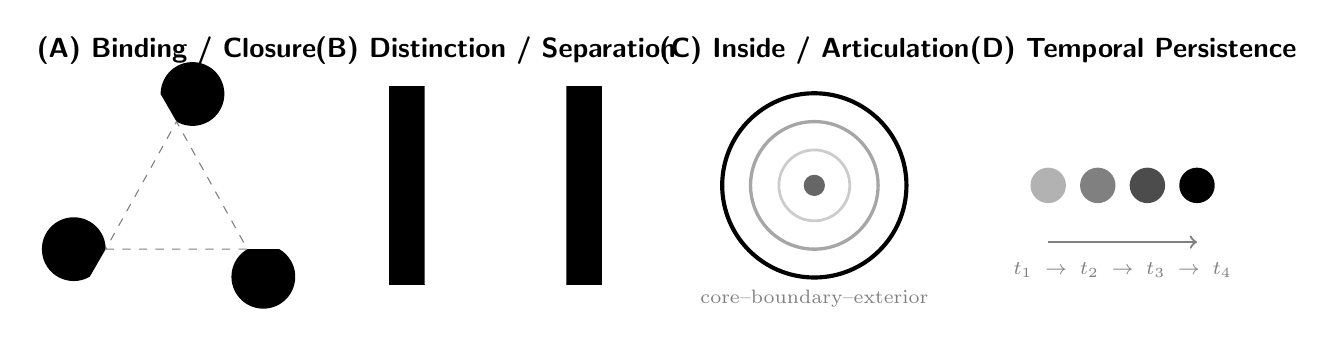
\begin{tikzpicture}[scale=0.9]
% Panel A: Kanizsa-style pac-men suggesting closure/binding
\begin{scope}[shift={(0,0)}]
\node[font=\sffamily\bfseries] at (1.5,3.3) {(A) Binding / Closure};
% Three pac-man shapes at triangle vertices
\foreach \a/\startang in {(0.5,0.5)/0, (2.5,0.5)/120, (1.5,2.3)/240} {
  \fill[black] \a arc[start angle=\startang, end angle=\startang+300, radius=0.45] -- cycle;
}
% Faint illusory triangle
\draw[gray, dashed, thin] (0.5,0.5) -- (2.5,0.5) -- (1.5,2.3) -- cycle;
\end{scope}

% Panel B: Vase-face silhouette (distinction/separation)
\begin{scope}[shift={(4.5,0)}]
\node[font=\sffamily\bfseries] at (1.5,3.3) {(B) Distinction / Separation};
% Simplified vase-face: two face profiles facing each other
\fill[black] (0,0) rectangle (0.5,2.8);
\fill[black] (2.5,0) rectangle (3,2.8);
% Curved face profiles
\fill[white] (0.5,0) .. controls (1.2,0.7) and (1.2,1.0) .. (0.8,1.4) .. controls (1.2,1.8) and (1.2,2.1) .. (0.5,2.8) -- (0.5,0);
\fill[white] (2.5,0) .. controls (1.8,0.7) and (1.8,1.0) .. (2.2,1.4) .. controls (1.8,1.8) and (1.8,2.1) .. (2.5,2.8) -- (2.5,0);
\end{scope}

% Panel C: Nested circles (morphological articulation / inside)
\begin{scope}[shift={(9,0)}]
\node[font=\sffamily\bfseries] at (1.5,3.3) {(C) Inside / Articulation};
\draw[line width=1.5pt] (1.5,1.4) circle (1.3);
\draw[line width=1.2pt, gray!70] (1.5,1.4) circle (0.9);
\draw[line width=1.0pt, gray!40] (1.5,1.4) circle (0.5);
\fill[black!60] (1.5,1.4) circle (0.15);
\node[font=\scriptsize, gray] at (1.5,-0.2) {core--boundary--exterior};
\end{scope}

% Panel D: Apparent motion dots with arrow (temporal persistence)
\begin{scope}[shift={(13.5,0)}]
\node[font=\sffamily\bfseries] at (1.5,3.3) {(D) Temporal Persistence};
\fill[black!30] (0.3,1.4) circle (0.25);
\fill[black!50] (1.0,1.4) circle (0.25);
\fill[black!70] (1.7,1.4) circle (0.25);
\fill[black] (2.4,1.4) circle (0.25);
\draw[->, thick, gray] (0.3,0.6) -- (2.4,0.6);
\node[font=\scriptsize, gray] at (1.35,0.2) {$t_1 \;\to\; t_2 \;\to\; t_3 \;\to\; t_4$};
\end{scope}
\end{tikzpicture}
\caption{The four structural requirements of SCC, illustrated through classical Gestalt phenomena. (A)~Pac-man inducers generate an illusory triangle through relational closure (Binding). (B)~The Rubin vase-face demonstrates figure-ground asymmetry (Distinction/Separation). (C)~Nested contours illustrate core-boundary-exterior stratification (Morphological Articulation). (D)~Apparent motion exemplifies structural inheritance across time (Temporal Persistence).}
\label{fig:gestalt}
\end{figure*}

% ============================================================
\section{The Formal Framework}
% ============================================================

We present the formal framework of SCC in terms accessible to cognitive scientists. Mathematical details that are not essential for understanding the conceptual structure are available in a companion mathematical paper; here we prioritize clarity and interpretive accessibility.

\subsection{The Cohesion Field}

The primitive entity of SCC is the \emph{cohesion field}:
\begin{equation}
u_t : X_t \to [0,1]
\end{equation}
where $X_t$ is a set of relational sites at time $t$ (positions in a visual field, neurons in a network, loci in any relational structure) and $u_t(x)$ is the degree to which site $x$ participates in a cohesive formation.

The cohesion field is not a probability of class membership, not a segmentation mask, and not a neural activation pattern---though it may be instantiated in neural activity. It is the intensity of \emph{cohesive participation}: how strongly a site is sustained by, and contributes to, the internal relational organization of a formation. A useful analogy: the field is like the pre-attentive ``togetherness'' that allows you to see a face in a crowd before you identify whose face it is.

The field takes values in the continuous interval $[0,1]$. This continuity is not a computational approximation of an underlying discrete state; it is the theory's foundational commitment. Pre-objective cohesion is intrinsically graded. Before a formation has stabilized into a recognizable object, some regions participate strongly, others weakly, and a boundary band of intermediate participation marks the transition.

\subsection{The Four Structural Requirements}

SCC formalizes four requirements that a cohesion field must satisfy to constitute a coherent pre-objective formation. These are not independent postulates chosen for convenience; they emerge from the analysis of what it means for a region of a relational space to hold together as a unit.

\subsubsection{Binding (Closure)}

A formation must be \emph{self-supporting}: the relational structure at each site must be consistent with the cohesion at that site. If a site has high cohesion, its relational neighbors should provide support for that cohesion; if it has low cohesion, high support from neighbors would be anomalous.

Formally, SCC defines a \emph{closure operator} $\mathrm{Cl}_t$ that takes the current cohesion field and computes what the field \emph{would be} if every site's cohesion were updated to reflect the support it receives from its relational neighborhood:
\begin{equation}
\mathrm{Cl}_t(u)(x) = \sigma\!\left(a_{\mathrm{cl}}\left[(1-\eta_{\mathrm{cl}})\,u(x) + \eta_{\mathrm{cl}}\,(P_t u)(x)\right] - \tau_{\mathrm{cl}}\right)
\end{equation}
where $\sigma$ is a sigmoid function, $(P_t u)(x) = \sum_y N_t(x,y)\,u(y)/z_x$ is the row-normalized neighborhood average, $\eta_{\mathrm{cl}} \in [0,1]$ balances self-retention against neighborhood aggregation, and $a_{\mathrm{cl}}, \tau_{\mathrm{cl}}$ are parameters (the companion paper~\cite{paper1} provides the full mathematical treatment).

A well-formed field is approximately a fixed point of its own closure: $\mathrm{Cl}_t(u) \approx u$. The degree to which this holds is measured by the \emph{binding predicate}:
\begin{equation}
\text{Bind}(u) = 1 - \frac{\|\mathrm{Cl}_t(u) - u\|_2}{\sqrt{n}}
\end{equation}
where $n = |X_t|$ is the number of sites. Bind $= 1$ means perfect self-support; Bind $= 0$ means the field is entirely inconsistent with its own relational structure. (The denominator $\sqrt{n}$ rather than $\|u\|_2$ ensures the measure is well-defined even for sparse fields and admits a proved bound: $\text{Bind} \geq 1 - \sqrt{\mathcal{E}_{\mathrm{cl}}/n}$, so small closure energy guarantees high binding.)

A crucial theoretical commitment: SCC's closure is \emph{contractive but not idempotent}. Applying closure twice does not give the same result as applying it once---repeated application converges progressively toward a fixed point. This means that closure is a \emph{process} with a trajectory, not an instantaneous projection. The trajectory carries information: different starting points may converge to different fixed points, and the rate of convergence reveals the stability of the formation.

This is the formal analogue of the Gestalt law of closure---incomplete figures are completed by the perceptual system---but with a critical refinement: completion is gradual and path-dependent, not all-or-nothing.

\subsubsection{Separation (Distinction)}

A formation must not only hold together internally; it must also \emph{distinguish itself from its surround}. A cohesive field that blends seamlessly into its background has binding but no separation---it is not yet a formation.

SCC formalizes distinction through the \emph{distinction operator} $D_t(x; 1-u)$, which measures the structural asymmetry between a site's interior support (from other high-cohesion sites) and its exterior support (from the complementary field $1-u$):
\begin{equation}
D_t(x; 1-u) = \sigma\!\left(a_D\!\left[\frac{\textstyle\sum_y N_t(x,y)\,u(y)}{\textstyle z_x} - \frac{\textstyle\sum_y N_t(x,y)\,(1-u(y))}{\textstyle z_x}\right]\right)
\end{equation}

The separation predicate measures how well the formation as a whole distinguishes itself from its surround:
\begin{equation}
\text{Sep}(u) = \frac{\sum_x u(x) \cdot D_t(x; 1-u)}{\sum_x u(x)}
\end{equation}
This is a $u$-weighted average of distinction: sites with higher cohesion contribute more to the separation score. This formulation avoids crisp thresholds and restricts the assessment to the formation's own support.

Crucially, the distinction operator is \emph{self-referential}: the field $u$ defines what counts as ``interior'' (high $u$) and ``exterior'' (high $1-u$), and then measures its own asymmetry against that self-defined partition. The field is both the object being evaluated and the standard against which it is evaluated. This self-referential character is not a technical curiosity---it is the formal expression of the idea that a formation distinguishes itself, rather than being distinguished by an external observer.

This is the formal analogue of the Gestalt figure-ground principle, but with a key addition: the figure-ground asymmetry is generated by the field's own structure, not imposed from outside.

\subsubsection{Morphological Articulation (Inside-Structure)}

A formation must have \emph{internal structure}: a core of deep interiority, a boundary band of transitional participation, and an exterior of non-participation. A featureless blob---uniformly high cohesion throughout---has binding but no morphological articulation.

SCC characterizes morphological quality using tools from topological data analysis. The \emph{superlevel-set filtration} of the cohesion field---the family of sets $\{x : u(x) \geq \theta\}$ as $\theta$ decreases from 1 to 0---reveals how the field's structure unfolds across thresholds. A well-articulated formation produces a single dominant connected component in its \emph{persistence diagram} (a tool from persistent homology that tracks the birth and death of topological features across thresholds).

The morphological quality measure is:
\begin{equation}
\mathcal{Q}_{\mathrm{morph}} = \frac{\ell_{\max} - \bar{u}}{1 - \bar{u}} \cdot \text{Artic}
\end{equation}
where $\ell_{\max}$ is the persistence (lifespan) of the longest-lived connected component, $\bar{u} = \sum u_i / n$ is the mean field value, and Artic measures the articulation ratio (how much the dominant component dominates all others). The normalization by $(1 - \bar{u})$ ensures that uniform fields yield $\mathcal{Q}_{\mathrm{morph}} = 0$ (axiom QM1: a featureless field has no morphological structure).

The Inside predicate is:
\begin{equation}
\text{Inside}(u) = \mathcal{Q}_{\mathrm{morph}}
\end{equation}

Inside $\approx 1$ means the field has a single, well-defined formation with clear core-to-boundary-to-exterior stratification. Inside $\approx 0$ means the field is topologically fragmented or lacks a coherent morphological profile.

\subsubsection{Temporal Persistence}

A formation must persist through time: its structurally significant core must be \emph{inherited} under temporal change. A formation that appears at one moment and vanishes entirely at the next has binding, separation, and inside-structure at a single time, but it is not yet a persisting entity.

SCC formalizes temporal persistence through a \emph{transport kernel} $M_{t \to s} : X_t \times X_s \to [0,1]$ that maps cohesive roles from time $t$ to time $s$. The value $M_{t \to s}(x,y)$ represents the degree to which the cohesive role of site $x$ at time $t$ is inherited by site $y$ at time $s$.

The persistence predicate measures whether the core of the formation at time $t$ is structurally preserved in the transported field at time $s$:
\begin{equation}
\text{Persist}(u_t, u_s, M) = \frac{|\mathrm{Core}_t \cap M^{-1}(\mathrm{Core}_s)|}{|\mathrm{Core}_t|}
\end{equation}

This simplified presentation uses crisp core sets for accessibility; the companion mathematical paper develops a soft transport formulation with quantitative bounds. We note that Persist is the least developed of the four predicates: the temporal theory has a proof strategy with partial results (three of six gaps closed), but no fully proved persistence theorem exists. The computational implementation includes both a core-overlap approximation and a transport-based \texttt{persist\_transport()} that implements the core-inheritance formula above using self-referential transport cost via cohesion fingerprints; in the weak transport regime, the self-referential fixed-point converges in 2--3 iterations.

\subsection{Non-Local Integration: The Co-Belonging Operator}
\label{sec:cobelonging}

The four structural requirements above rely on local relational structure---adjacency between neighboring sites. But perceptual organization often exhibits \emph{non-local} coherence: elements that are spatially separated can nonetheless belong together, not because they are adjacent but because they are linked through a chain of mutually supporting intermediate sites. The Gestalt principle of common fate captures this intuition: elements that share a common dynamic or structural role co-belong, even at a distance.

SCC formalizes non-local integration through the \emph{co-belonging operator} $C_t : X_t \times X_t \to [0,\infty)$, which measures the degree to which two sites participate in the same cohesive formation. The provisional realization takes the resolvent form:
\begin{equation}
C_t = (I - \alpha\, W_{\mathrm{sym}})^{-1}
\end{equation}
where $W_{\mathrm{sym}}$ is a symmetrized cohesion-weighted adjacency matrix (with entries $W_{\mathrm{sym}}(x,y) = \sqrt{u_t(x)}\, N_t(x,y)\, \sqrt{u_t(y)} / d_x$ for degree normalization $d_x$) and $\alpha > 0$ controls the range of integration.

The resolvent has an illuminating series expansion:
\begin{equation}
C_t = \sum_{k=0}^{\infty} \alpha^k W_{\mathrm{sym}}^k = I + \alpha\, W_{\mathrm{sym}} + \alpha^2 W_{\mathrm{sym}}^2 + \cdots
\end{equation}
Each term captures the contribution of paths of length $k$ through the cohesion-weighted relational graph. The identity term ($k=0$) registers each site's self-co-belonging. The first-order term ($k=1$) captures direct neighbors, weighted by cohesion. Higher-order terms capture progressively longer chains of mutual support. The series converges when $\alpha\, \rho(W_{\mathrm{sym}}) < 1$, where $\rho$ denotes the spectral radius.

Why a resolvent rather than simple adjacency? Consider two sites on opposite sides of a cohesive formation. They are not adjacent, yet they co-belong---they participate in the same structural whole. The resolvent captures this: their co-belonging score integrates over \emph{all} paths of mutual support connecting them, weighted by the cohesion along each path. Two sites may co-belong without being adjacent (if linked through a chain of high-cohesion intermediaries), and two adjacent sites may fail to co-belong (if they lie on opposite sides of a cohesive boundary, with low cohesion between them).

Co-belonging serves a diagnostic role---identifying which sites are structurally integrated into the formation---but does not enter the energy functional directly. This architectural choice keeps the energy analytically tractable. (The separation predicate $\text{Sep}$ uses $u(x)$ as an importance weight, restricting the assessment to the formation's own support.)

\subsection{The Diagnostic Vector}

The four structural requirements define a continuous diagnostic vector:
\begin{equation}
\mathbf{d} = (\text{Bind}, \text{Sep}, \text{Inside}, \text{Persist}) \in [0,1]^4
\end{equation}

This vector replaces the single scalar of Gestalt Pr\"{a}gnanz with a decomposed assessment. A formation with $\mathbf{d} = (0.95, 0.30, 0.80, 0.70)$ is well-bound but poorly separated---diagnostic information that would be lost in a single ``goodness'' score. The diagnostic vector makes the \emph{profile} of formation quality visible: which requirements are satisfied, which are deficient, and to what degree (Fig.~\ref{fig:radar}).

The four components are \emph{conceptually independent}: each can in principle be manipulated independently of the others. A formation can have high binding but low separation (a region that holds together internally but fades into its surround), or high separation but low inside-structure (a region sharply distinct from its background but internally uniform). This independence is a central prediction of the theory (see Section~V).

\begin{figure}[!t]
\centering
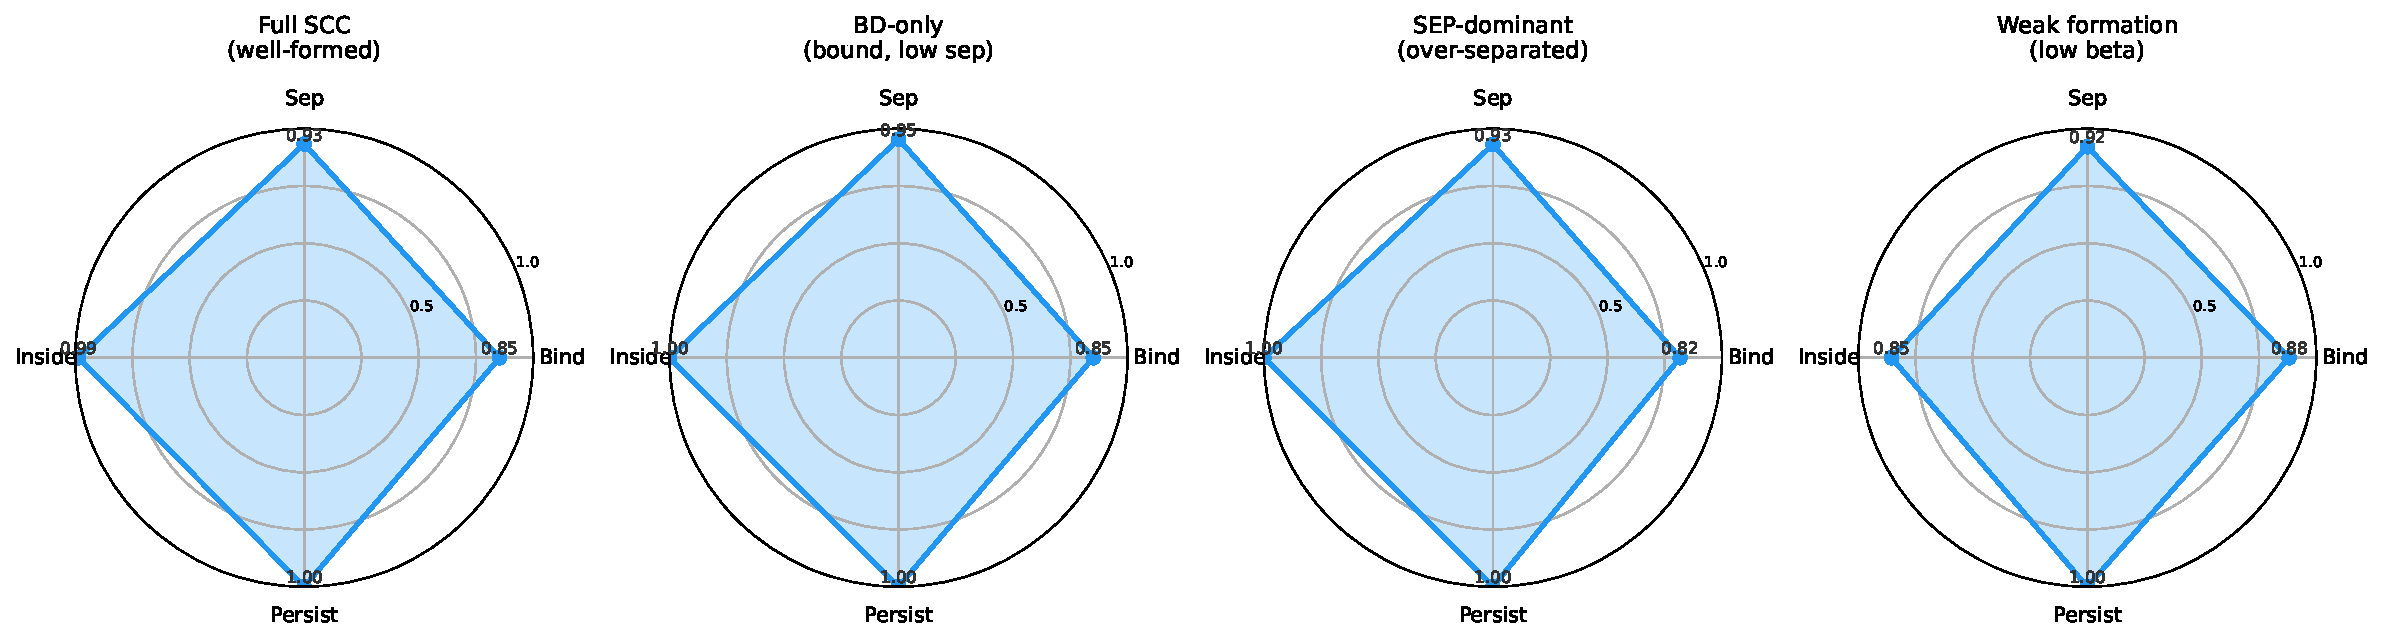
\includegraphics[width=\columnwidth]{figures/fig2_radar.pdf}
\caption{Diagnostic vectors for four formation types: well-formed (full SCC), bound-only (BD), over-separated (SEP-dominant), and weak formation. Each axis shows one component of the diagnostic vector $\mathbf{d} \in [0,1]^4$.}
\label{fig:radar}
\end{figure}

\subsection{The Energy Principle}

What makes a cohesion field settle into a particular configuration rather than any other? SCC answers this through a variational principle: formations are (meta)stable configurations that minimize an energy functional encoding all four structural requirements. Each energy term penalizes a specific kind of structural deficiency.

\emph{Closure energy} penalizes self-inconsistency---the discrepancy between the field and its own relational completion:
\begin{equation}
\label{eq:ecl}
\mathcal{E}_{\mathrm{cl}}(u) = \sum_x \big(\mathrm{Cl}_t(u)(x) - u(x)\big)^2
\end{equation}
A field that perfectly sustains itself under closure pays zero closure cost.

\emph{Separation energy} penalizes cohesive sites that fail to distinguish themselves from the exterior:
\begin{equation}
\label{eq:esep}
\mathcal{E}_{\mathrm{sep}}(u) = \sum_x u(x)\,\big(1 - D_t(x; 1-u)\big)
\end{equation}
Sites with high cohesion ($u \approx 1$) but low distinction ($D_t \approx 0$) contribute heavily---they are ``trying to belong'' without being structurally differentiated.

\emph{Boundary/morphology energy} enforces spatial coherence and penalizes featureless intermediate states:
\begin{equation}
\label{eq:ebd}
\mathcal{E}_{\mathrm{bd}}(u) = \alpha \!\sum_{x,y} N_t(x,y)\big(u(x) - u(y)\big)^2 + \beta \sum_x u(x)^2\big(1 - u(x)\big)^2
\end{equation}
The first sub-term is a smoothness penalty: it discourages erratic oscillation by penalizing large differences between neighboring sites. The second is a \emph{double-well potential}: it penalizes intermediate cohesion values, favoring fields that commit to either full participation ($u \approx 1$) or non-participation ($u \approx 0$). Together, these drive the field toward well-defined interior regions, coherent boundary bands, and clear exterior---the morphological signature of a genuine formation.

\emph{Transport energy} penalizes temporal discontinuity in cohesive organization:
\begin{equation}
\label{eq:etr}
\mathcal{E}_{\mathrm{tr}}(u_t, u_s) = \!\sum_{x,y} M_{t \to s}(x,y)\,\omega(u_t(x), u_s(y))\big(u_s(y) - u_t(x)\big)^2
\end{equation}
where $\omega$ weights high-cohesion sites more heavily. A formation whose core is smoothly inherited from one moment to the next pays low transport cost.

The full energy is a weighted combination of all four terms:
\begin{equation}
\label{eq:energy}
\mathcal{E}(u) = \lambda_{\mathrm{cl}}\,\mathcal{E}_{\mathrm{cl}} + \lambda_{\mathrm{sep}}\,\mathcal{E}_{\mathrm{sep}} + \lambda_{\mathrm{bd}}\,\mathcal{E}_{\mathrm{bd}} + \lambda_{\mathrm{tr}}\,\mathcal{E}_{\mathrm{tr}}
\end{equation}
The four terms are conceptually independent: each addresses a logically separable structural requirement. A field may be closed but undistinguished, distinguished but morphologically incoherent, morphologically coherent but temporally discontinuous. The relative weights $\lambda_{\mathrm{cl}}, \lambda_{\mathrm{sep}}, \lambda_{\mathrm{bd}}, \lambda_{\mathrm{tr}}$ control the balance among requirements---and the ``competition'' between Gestalt principles (sometimes proximity dominates, sometimes common fate) is formalized as the interplay of these weights.

\subsubsection{The Volume Constraint}

The energy is minimized subject to a structural constraint on total cohesion:
\begin{equation}
\sum_{x \in X_t} u_t(x) = m
\end{equation}
where $m > 0$ is the \emph{cohesive budget}. This constraint is not a computational convenience but an ontological commitment: any finite relational system has finite capacity to sustain cohesion. Universal cohesion ($u \equiv 1$ everywhere) is as featureless as universal non-cohesion ($u \equiv 0$)---both lack the selectivity that makes formation possible. The cohesive budget $m$ is the finite resource that \emph{forces} selectivity, and selectivity is the precondition for formation.

Without this constraint, the trivial field $u \equiv 0$ globally minimizes all energy terms (since every term is nonnegative and vanishes at zero). The volume constraint is therefore mathematically necessary for the existence of non-trivial formations. Formations are the (meta)stable critical points of the energy on the constraint manifold---cohesion field configurations that represent balanced compromises among self-support, self-distinction, morphological regularity, and temporal continuity.

\subsection{Self-Referential Structure}

The formal architecture of SCC has a distinctive self-referential character that distinguishes it from all standard variational frameworks. The cohesion field $u$ defines three operators---closure $\mathrm{Cl}_t$, distinction $D_t$, and co-belonging $C_t$---each of which depends on $u$ itself. Two of these modes (self-completion and self-contrast) enter the energy functional directly; the third (self-integration via $C_t$) enters the diagnostic predicates but not the energy---an architectural decision, not an oversight. The self-referential structure thus operates through two variational modes and one diagnostic mode. These operators define the energy functional whose minimization determines $u$:
\begin{equation*}
u \xrightarrow{\text{defines}} (\mathrm{Cl}_t, D_t) \xrightarrow{\text{defines}} \mathcal{E} \xrightarrow{\text{determines}} u \qquad (\text{also: } u \to C_t \to \text{diagnostics})
\end{equation*}

An accessible analogy: consider a social group that defines its own membership criteria (``people who share our values''), evaluates itself against those criteria (``do our current members actually share these values?''), and adjusts both its membership and its criteria in response. The criteria and the group co-evolve. In SCC, the cohesion field plays both roles: it defines the operators (the membership criteria), and it is the entity evaluated by those operators (the group). The field is simultaneously the standard and the thing measured against the standard.

This loop is not circular in definition---the energy is a well-defined function of $u$ at every point---but it is circular in computation: updating $u$ changes the operators, which change the energy landscape, which changes the optimal $u$. The distinction between \emph{definitional acyclicity} (no circular definitions) and \emph{computational cyclicity} (iterative self-consistency) is essential.

The self-referential structure exhibits \emph{operational closure} in the sense described by Maturana and Varela \cite{maturana1980autopoiesis}: the criteria by which the field is evaluated are defined by the field itself, rather than imposed externally. We note that this is weaker than full autopoiesis, which requires self-production of components---here the operator forms and parameters are externally given; only their numerical values depend on the field (Fig.~\ref{fig:loop}). Cut any link in the loop by inserting external data---external adjacency weights, externally defined labels, external tracking identifiers---and the theory reduces to standard segmentation, classification, or tracking. Keep the loop closed, and you have SCC.

\begin{figure}[!t]
\centering
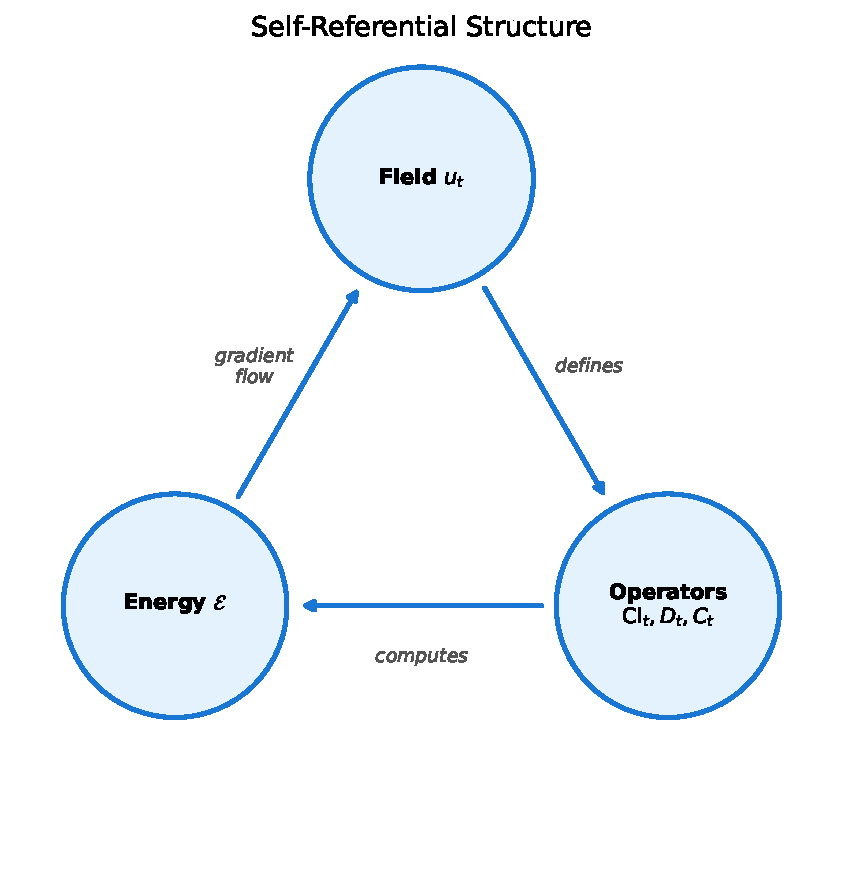
\includegraphics[width=\columnwidth]{figures/fig5_loop.pdf}
\caption{The self-referential structure of SCC. The cohesion field defines the operators; the operators define the energy; energy minimization determines the field.}
\label{fig:loop}
\end{figure}


% ============================================================
\section{The Gestalt Connection}
% ============================================================

The Gestalt psychologists described the pre-objective organization of the perceptual field with extraordinary precision, but they never succeeded in providing a unified formal framework for their insights. SCC provides such a framework. The correspondence between SCC's formal apparatus and the classical Gestalt laws is structural rather than merely metaphorical: each Gestalt principle maps onto a specific formal operator or theorem. We emphasize, however, that these are structural analogies within a unified variational framework, not direct formalizations of the specific perceptual phenomena (illusory contour completion, border ownership, synchronous motion grouping) that the Gestalt psychologists described.

\subsection{Mapping Gestalt Laws to SCC Operators}

Table~\ref{tab:gestalt} presents the structural mapping between Gestalt principles and SCC constructs. The alignment is not accidental---SCC was designed to formalize the pre-objective level of perceptual organization that Gestalt psychology described phenomenologically.

\begin{table}[!t]
\centering
\caption{Structural Mapping: Gestalt Principles to SCC Formalism}
\label{tab:gestalt}
\begin{tabular}{p{2.2cm}p{2.8cm}p{2.2cm}}
\toprule
\textbf{Gestalt Principle} & \textbf{SCC Counterpart} & \textbf{Status} \\
\midrule
Closure (Geschlossen\-heit) & $\mathrm{Cl}_t$ (closure operator) & Structural analogue \\
\addlinespace
Proximity (N\"{a}he) & $N_t$ (adjacency kernel) & Direct formalization \\
\addlinespace
Similarity / Common Fate & $C_t$ (co-belonging, diagnostic) & Structural analogue (non-local) \\
\addlinespace
Figure-Ground & $D_t$ (distinction operator) & Structural analogue \\
\addlinespace
Good Continuation & $T_t$ (transition operator) & Open problem---no formal operator \\
\addlinespace
Pr\"{a}gnanz & Metastable energy minima & Variational analogue \\
\addlinespace
Common Fate (temporal) & $M_{t \to s}$ (transport kernel) & Structural analogue (inheritance, not co-motion) \\
\bottomrule
\end{tabular}
\end{table}

Several features of this mapping deserve comment. First, the mapping is \emph{many-to-one} in the sense that multiple Gestalt principles correspond to distinct aspects of a single variational framework. The Gestalt laws are not independent heuristics in SCC; they are consequences of a unified energy minimization principle operating through the operator pair.

Second, SCC \emph{extends} the Gestalt framework in several directions. The co-belonging operator $C_t$ generalizes similarity and common fate to a non-local integration principle: two sites can co-belong even if they are not spatially adjacent, provided they are linked through a chain of mutually supporting intermediate sites. The diagnostic vector $\mathbf{d} \in [0,1]^4$ replaces the single scalar of Pr\"{a}gnanz with a decomposed assessment. And the self-referential energy provides dynamics (gradient flow) that the Gestalt description lacked.

Third, one Gestalt principle---good continuation---has only conceptual alignment with SCC. The transition operator $T_t$ remains an open theoretical problem: its formal specification and axiomatization have not been completed. This is an honest gap.

\subsection{Three Gestalt Puzzles SCC Resolves}

Beyond mapping, SCC resolves three long-standing puzzles in the Gestalt tradition.

\subsubsection{Why Is Pr\"{a}gnanz Metastable, Not Optimal?}

The classical Gestalt notion of Pr\"{a}gnanz suggests that perception tends toward the ``best'' possible organization---the most regular, most symmetric, most stable configuration. But perception sometimes settles into demonstrably suboptimal organizations. The Necker cube has two stable percepts, neither of which is globally optimal; the duck-rabbit figure has two equally valid interpretations. If Pr\"{a}gnanz were global optimality, such ambiguity would be impossible.

SCC resolves this: formations are \emph{metastable} local minima of the energy, not global optima. Each metastable formation occupies an energy basin with enhanced stability barriers (this is a mathematical theorem---Theorem~4 in the companion paper~\cite{paper1}). The ``goodness'' that Pr\"{a}gnanz captures is \emph{local} goodness: stability within a basin, resistance to perturbation, not global superiority. The energy landscape can contain multiple metastable basins of comparable depth, producing the bistability that Gestalt psychology described but could not explain formally.

Moreover, the self-referential closure operator enhances local stability beyond what a standard (non-self-referential) energy would produce. The mathematical result (Theorem~4 of~\cite{paper1}) shows that the closure term contributes a strictly positive-definite Hessian correction---every energy basin in SCC has a strictly larger minimum Hessian eigenvalue than the corresponding basin in a standard Allen-Cahn model, indicating greater local curvature at the minimizer. This enhanced metastability predicts measurably longer dwell times in perceptual rivalry (see Prediction~3 in Section~V).

\subsubsection{Why Does Perceptual History Matter?}

Adaptation, priming, and sequential effects influence perceptual organization: the same stimulus may be organized differently depending on what preceded it \cite{leopold2002stable}. Equilibrium theories that predict perception from the current stimulus alone cannot account for these history effects.

SCC explains history dependence through \emph{non-idempotent closure}. Because applying closure twice is not the same as applying it once---because closure is a contractive process, not a projective one---the \emph{trajectory} of perceptual organization carries information. Different starting points (different adaptation histories) follow different convergence paths through the energy landscape, and these paths may converge to \emph{different} metastable formations. Path dependence is not a nuisance in SCC; it is a structural consequence of the theory's commitment to non-idempotent closure.

This is a foundational commitment, not an adjustable parameter. The theory deliberately omits idempotence as a primitive axiom of closure, and this omission has mathematical consequences: it yields strictly positive-definite Hessian contributions (Theorem~2 of~\cite{paper1}) that would be only semidefinite under idempotent closure. The mathematical advantage of non-idempotence---stronger local stability, larger Hessian curvature, richer dynamics---provides formal support for what is ultimately a philosophical commitment: that formation is a process, not a state.

\subsubsection{Why Is Figure-Ground Asymmetric?}

Rubin \cite{rubin1921visuell} observed that figure-ground segregation is inherently asymmetric: the figure ``owns'' its boundary in a way that the ground does not. The boundary between figure and ground belongs perceptually to the figure. This asymmetry is phenomenologically robust but has resisted formal explanation.

SCC's distinction operator $D_t(x; 1-u)$ is structurally asymmetric by construction. It measures the excess of interior relational support over exterior relational support at each site. At the boundary of a formation, interior sites (high $u$) contribute more to the local support average than exterior sites (low $u$), creating an inherent asymmetry: the boundary is ``seen from'' the interior, not from the exterior. The formation's boundary belongs to the formation because the distinction operator evaluates it from the formation's perspective---the self-referential perspective defined by the field itself.

\subsection{What SCC Adds Beyond Gestalt Description}

The relationship between SCC and Gestalt psychology is not one of formalization alone. SCC adds three elements that the Gestalt tradition lacked:

\begin{enumerate}
\item \textbf{Quantitative, continuous measures.} Where Gestalt provides qualitative laws (``similar things group together''), SCC provides continuous-valued operators ($C_t(x,y)$ quantifies the degree of co-belonging between any two sites) and a four-dimensional diagnostic vector that can be computed for any cohesion field.

\item \textbf{A unifying variational principle.} Where Gestalt provides a list of independent principles (proximity, similarity, closure, etc.), SCC derives them as consequences of a single energy functional (\ref{eq:energy}). The ``competition'' between Gestalt principles---sometimes proximity wins, sometimes similarity wins---is formalized as the interplay of energy terms with different relative weights.

\item \textbf{Temporal persistence.} The Gestalt tradition had no formal account of how a perceptual organization maintains its identity through time. SCC's transport kernel $M_{t \to s}$ formalizes the temporal dimension: the persistence predicate measures whether the formation's core is structurally inherited across time, providing a formal account of perceptual identity.
\end{enumerate}


% ============================================================
\section{Distinguishing SCC from Contemporary Theories}
% ============================================================

SCC operates at a different level of description than most contemporary theories of perception and consciousness. It is essential to characterize the relationship precisely: SCC is \emph{complementary} to these theories, not competing with them at the same level.

\subsection{SCC vs.\ Predictive Processing}

Predictive Processing (PP) \cite{clark2013whatever,friston2010free,hohwy2013predictive} proposes that the brain is a prediction machine: it maintains a hierarchical generative model of the external world and continuously updates its predictions to minimize prediction error. PP has been enormously productive in explaining perceptual phenomena, from illusions to attention to action.

\begin{table}[!t]
\centering
\caption{Comparison: SCC vs.\ Predictive Processing}
\label{tab:pp}
\begin{tabular}{p{2.2cm}p{2.8cm}p{2.5cm}}
\toprule
\textbf{Dimension} & \textbf{SCC} & \textbf{PP} \\
\midrule
Ontological level & Pre-objective (before objects) & Post-objective (beliefs about objects) \\
\addlinespace
Generative model & Internal (field predicts itself) & External (model predicts sensory data) \\
\addlinespace
Self-reference & Structural (operator pair) & Present in FEP; absent in hierarchical PP \\
\addlinespace
Direction & Energy minimization on cohesion field & Top-down prediction + bottom-up error (hierarchical PP); self-organization (FEP) \\
\addlinespace
Core mechanism & Energy minimization on cohesion field & Free energy minimization on beliefs \\
\bottomrule
\end{tabular}
\end{table}

The key distinction (Table~\ref{tab:pp}) is one of \emph{level of description}. PP is epistemological: it models how an agent updates its beliefs about the external world. SCC is structural: it provides a framework for characterizing graded formation states that are formally richer than the discrete-object representations PP typically operates on. The two are complementary: SCC provides a \emph{substrate description} in which formation properties are decomposed and graded, while PP interprets, categorizes, and predicts at the object level.

There is, however, a structural analogy. SCC's closure energy $\|\mathrm{Cl}(u) - u\|^2$ has the form of a prediction error: the field ``predicts'' its own relational completion and is penalized for the discrepancy. But unlike PP's prediction error, SCC's error is \emph{self-referential}: the ``prediction'' ($\mathrm{Cl}(u)$) and the ``data'' ($u$) are aspects of the same field. There is no external sensory signal. The field is testing itself against its own self-generated standard.

\textbf{Testable difference.} Hierarchical PP predicts that top-down predictions drive perceptual organization. SCC predicts that basic coherence emerges from the operator pair's self-referential energy minimization. These make different predictions about the time course of perceptual grouping: if SCC is correct, figure-ground segregation (measurable via the N1 EEG component) should \emph{precede} top-down categorical effects (N2/P300). We acknowledge that active inference frameworks \cite{friston2010free} do address aspects of self-organization and perceptual grouping; SCC targets a more foundational structural level.

\subsection{SCC vs.\ Global Workspace Theory}

Global Workspace Theory (GWT) \cite{baars1988cognitive,dehaene2011experimental} proposes that consciousness arises when information is broadcast to a global workspace accessible to multiple specialized processors.

\begin{table}[!t]
\centering
\caption{Comparison: SCC vs.\ Global Workspace Theory}
\label{tab:gwt}
\begin{tabular}{p{2.2cm}p{2.8cm}p{2.5cm}}
\toprule
\textbf{Dimension} & \textbf{SCC} & \textbf{GWT} \\
\midrule
Starting point & Graded cohesion field & Discrete contents in modules \\
\addlinespace
Competition & Energy landscape (metastable basins) & Contents compete for workspace access \\
\addlinespace
Consciousness & Not addressed (pre-objective level) & Workspace access $=$ consciousness \\
\addlinespace
Scope & Formation emergence & Information broadcasting \\
\bottomrule
\end{tabular}
\end{table}

The key distinction (Table~\ref{tab:gwt}): GWT assumes contents are \emph{already discrete}---they compete for broadcasting. SCC asks how contents become discrete in the first place. SCC operates at a level \emph{prior} to GWT's starting point.

\textbf{Testable difference.} GWT predicts all-or-nothing access: contents are either in the workspace or not. SCC predicts graded formation quality with continuous transitions. Non-conscious stimuli should still have measurable diagnostic vector components---partial binding, partial separation---indicating formations that have not fully stabilized, not absent representations.

\subsection{SCC vs.\ Integrated Information Theory}

Integrated Information Theory (IIT) \cite{tononi2004information,oizumi2014phenomenology} defines consciousness in terms of integrated information $\Phi$ computed over a system decomposed into elements.

\begin{table}[!t]
\centering
\caption{Comparison: SCC vs.\ Integrated Information Theory}
\label{tab:iit}
\begin{tabular}{p{2.2cm}p{2.8cm}p{2.5cm}}
\toprule
\textbf{Dimension} & \textbf{SCC} & \textbf{IIT} \\
\midrule
Primitive & Cohesion field (continuous) & Causal relations among discrete elements \\
\addlinespace
Integration measure & $C_t$ (field-dependent co-belonging) & $\Phi$ (over system partition) \\
\addlinespace
Level & Pre-objective & System-level \\
\addlinespace
Consciousness claims & None & $\Phi > 0$ implies consciousness \\
\bottomrule
\end{tabular}
\end{table}

The distinction (Table~\ref{tab:iit}): IIT presupposes individuation---the system must be decomposed into elements before $\Phi$ can be computed. SCC describes individuation in progress. IIT asks how much a system's interactions exceed the sum of its parts; SCC asks how parts come to cohere into a system.

\textbf{Testable difference.} IIT's $\Phi$ is a single scalar. SCC's diagnostic vector is four-dimensional. Formations can be highly integrated (high co-belonging $C_t$) but poorly distinguished (low Sep)---a state that IIT's single scalar cannot represent.

\subsection{SCC vs.\ Bayesian Brain}

Bayesian brain accounts \cite{knill2004bayesian,lee2003hierarchical} model perception as approximate inference over a generative model with variables for objects and features.

\begin{table}[!t]
\centering
\caption{Comparison: SCC vs.\ Bayesian Brain}
\label{tab:bayesian}
\begin{tabular}{p{2.2cm}p{2.8cm}p{2.5cm}}
\toprule
\textbf{Dimension} & \textbf{SCC} & \textbf{Bayesian} \\
\midrule
Prediction error & Self-referential ($u$ vs.\ $\mathrm{Cl}(u)$) & External (prediction vs.\ sensation) \\
\addlinespace
Priors & Emergent from energy landscape & Explicit in generative model \\
\addlinespace
Formation & Energy minimization discovers structure & Inference assumes structure \\
\bottomrule
\end{tabular}
\end{table}

The distinction (Table~\ref{tab:bayesian}): Bayesian approaches presuppose a generative model with variables corresponding to objects. SCC asks how the perceptual system arrives at its variables---how it carves the sensory flux into the joints that Bayesian inference then exploits. SCC is \emph{pre-Bayesian}: it operates at the level where the categories for Bayesian inference are being constituted.

\textbf{Testable difference.} Bayesian models predict contractive updating toward a single posterior. SCC predicts multiple metastable formations with path-dependent selection. For ambiguous stimuli, Bayesian models predict smooth probability distributions over interpretations; SCC predicts discrete metastable states with enhanced dwell times.

\subsection{Summary of Positioning}

SCC is not a theory of everything. It is a theory of \emph{structural formation}---a framework for characterizing how coherent somethings organize within a graded field, with properties (binding, separation, articulation, persistence) that can be assessed independently and continuously. It does not compete with PP, GWT, IIT, or Bayesian brain at their respective levels; it provides a structurally richer description of the formation states that these theories typically take as given.


% ============================================================
\section{Empirical Predictions}
% ============================================================

SCC generates ten empirical predictions organized by domain and testability. These predictions are \emph{derived from the theory}, not added post hoc; each follows from a specific formal result or structural property.

\subsection{Cognitive and Perceptual Predictions}

\textbf{P1: Closure is contractive, not projective.} SCC's non-idempotent closure predicts that perceptual completion is a gradual, progressive process, not an all-or-nothing operation. In ambiguous displays (Kanizsa triangles, amodal completion), repeated brief exposure should produce progressively more stable percepts---contractive convergence rather than sudden completion.

\emph{Protocol:} Priming paradigms with varying exposure durations; measure completion strength via EEG steady-state responses. \emph{Distinguishes from:} Bayesian models (probabilistic updating) and equilibrium models (all-or-nothing completion). \emph{Testability:} \textbf{HIGH}---standard psychophysics and EEG.

\textbf{P2: Perceptual organization has four independent dimensions.} The diagnostic vector $\mathbf{d} \in [0,1]^4$ predicts that binding, separation, inside-structure, and persistence are independently manipulable perceptual dimensions.

\emph{Protocol:} Factorial manipulation of stimulus properties: internal coherence (Bind), figure-ground contrast (Sep), shape complexity (Inside), temporal continuity (Persist). If four-term independence holds, the four factors should show no interactions (or specific, predictable interactions). \emph{Distinguishes from:} Single-scalar models (Pr\"{a}gnanz, posterior probability). \emph{Testability:} \textbf{HIGH}---standard psychophysics with factor analysis.

\textbf{P3: Metastable percepts have longer dwell times than equilibrium models predict.} The self-referential closure energy deepens energy basins beyond what standard models predict (Theorem~4 of~\cite{paper1}), implying systematically longer dwell times in perceptual rivalry. \emph{Computational validation:} Langevin escape experiments confirm this prediction---SCC formations survived noise in 24/30 trials (80\%) vs.\ 16/30 (53\%) for Allen--Cahn alone ($p = 0.037$, Fisher exact test). A temperature sweep shows SCC maintains higher binding at all noise levels ($+0.006$ to $+0.029$ mean Bind advantage).

\emph{Protocol:} Binocular rivalry with quantitative model comparison: Allen-Cahn model (standard barriers) vs.\ SCC model (enhanced barriers from self-referential closure). \emph{Distinguishes from:} Standard energy-based rivalry models. \emph{Testability:} \textbf{MEDIUM}---requires quantitative model fitting.

\textbf{P4: Perceptual history affects current organization.} Non-idempotent closure predicts that the adaptation \emph{trajectory}---not just the final adapted state---influences the percept for ambiguous stimuli.

\emph{Protocol:} Present ambiguous stimuli after different adaptation sequences (same endpoint, different paths). \emph{Distinguishes from:} Equilibrium models where only current input matters. \emph{Testability:} \textbf{HIGH}---standard psychophysics; some existing data supports this \cite{leopold2002stable}.

\textbf{P5: Self-referential distinction precedes object recognition.} SCC predicts that figure-ground segregation (driven by the self-referential distinction operator) occurs \emph{before} top-down categorical effects.

\emph{Protocol:} Rapid serial visual presentation (RSVP); measure time course of figure-ground segregation (N1 EEG component) vs.\ object identification (N2/P300). \emph{Distinguishes from:} Predictive processing, which predicts top-down prediction precedes segregation. \emph{Testability:} \textbf{HIGH}---standard ERP paradigm.

\subsection{Biological Predictions}

\textbf{P6: Morphogenetic boundaries follow a Bind $\to$ Sep $\to$ Inside developmental order.} In developing embryos, newly forming tissue boundaries should show high Bind (self-support) first, then high Sep (sharp distinction), with Inside (morphological articulation) emerging last.

\emph{Domain:} Developmental biology (e.g., zebrafish somitogenesis). \emph{Method:} Spatial transcriptomics at tissue boundaries across developmental stages. \emph{Testability:} \textbf{MEDIUM}---requires spatial transcriptomics with SCC model fitting.

\textbf{P7: Self-referential binding prolongs biomolecular condensate lifetimes.} In cells, biomolecular condensates whose components bind preferentially to condensates containing themselves (self-referential binding) should be longer-lived than predicted by classical phase separation models.

\emph{Domain:} Cellular biology (liquid-liquid phase separation). \emph{Method:} FRAP experiments comparing self-referential vs.\ non-self-referential condensate components. \emph{Testability:} \textbf{MEDIUM}---requires specific experimental design.

\textbf{P8: Neural assemblies show formation dynamics, not clustering dynamics.} Neural assemblies identified by SCC should exhibit the four-predicate structure (Bind, Sep, Inside, Persist). ``Proto-assemblies'' with high Bind but low Sep should exist before stimulus onset and be recruited by stimuli.

\emph{Domain:} Systems neuroscience. \emph{Method:} Multi-electrode recordings with SCC diagnostic analysis. \emph{Testability:} \textbf{MEDIUM-HIGH}---re-analysis of existing datasets is possible.

\subsection{Materials and Physics Predictions}

\textbf{P9: Modified coarsening exponents in self-referential phase separation.} In systems where the local order parameter affects its own energetic contribution, SCC predicts modified coarsening rates $R(t) \sim t^{1/3 + \delta}$ where $\delta$ depends on self-referential coupling strength.

\emph{Method:} STEM time-series of spinodal decomposition. \emph{Testability:} \textbf{LOW}---requires specialized materials and high-resolution imaging.

\textbf{P10: Self-referential surface tension in the sharp-interface limit.} SCC's $\Gamma$-convergence theorem predicts a modified surface tension $\sigma_{\mathrm{eff}} = \sigma_{\mathrm{AC}} + \delta\sigma(\lambda_{\mathrm{cl}}, \lambda_{\mathrm{sep}})$.

\emph{Method:} Contact angle or capillary length experiments in systems with concentration-dependent interfacial properties. \emph{Testability:} \textbf{LOW}---requires precise surface tension measurement.

\subsection{Summary of Predictions}

Table~\ref{tab:predictions} summarizes all ten predictions with their testability ratings, the theories from which they distinguish SCC, and computational validation status where available. Five predictions have received computational validation: P1 (contraction rate $0.851 < 0.875$, confirmed), P2 (partially confirmed: closure$\to$Bind and separation$\to$Sep coupling verified, full $4\times4$ independence requires further work), P3 (confirmed: $1.5\times$ survival advantage under noise, $p = 0.037$), P4 (confirmed: 96\% of initialization pairs yield distinct formations), and P5 (confirmed: Sep exceeds $0.5$ at step~0, Inside only at step~200).

\begin{table*}[!t]
\centering
\caption{Summary of Empirical Predictions. Computational validation column indicates results from graph-based simulations (not perceptual experiments).}
\label{tab:predictions}
\begin{tabular}{clp{2.6cm}cp{2.2cm}p{2.5cm}p{1.8cm}}
\toprule
\textbf{\#} & \textbf{Domain} & \textbf{Prediction} & \textbf{Testability} & \textbf{Method} & \textbf{Distinguishes From} & \textbf{Comp.\ Valid.} \\
\midrule
P1 & Perception & Closure is contractive, not projective & HIGH & Priming + EEG & Bayesian, equilibrium & Confirmed \\
P2 & Perception & Organization has 4 independent dims & HIGH & Factorial psychophysics & Single-scalar (Pr\"{a}gnanz) & Partial \\
P3 & Perception & Enhanced dwell times in rivalry & MEDIUM & Rivalry + model fit & Energy-barrier models & Confirmed \\
P4 & Perception & Adaptation trajectory affects percept & HIGH & Bistable figures & Equilibrium models & Confirmed \\
P5 & Perception & Distinction precedes recognition & HIGH & RSVP + ERP & Predictive processing & Confirmed \\
\addlinespace
P6 & Biology & Bind$\to$Sep$\to$Inside order & MEDIUM & Spatial transcriptomics & Turing patterns & --- \\
P7 & Biology & Self-ref.\ binding extends condensate life & MEDIUM & FRAP experiments & Classical Cahn-Hilliard & --- \\
P8 & Neuroscience & Assemblies have 4-predicate structure & MED-HIGH & Multi-electrode + SCC & ICA/NMF clustering & --- \\
\addlinespace
P9 & Physics & Modified coarsening exponents & LOW & STEM time-series & Lifshitz-Slyozov-Wagner & --- \\
P10 & Physics & Self-referential surface tension & LOW & Contact angle & Standard Modica-Mortola & --- \\
\bottomrule
\end{tabular}
\end{table*}


% ============================================================
\section{Computational Proof-of-Concept}
% ============================================================

To demonstrate that the formal framework is not merely a philosophical proposal but a mathematically tractable theory, we report computational experiments that validate the core claims: formations emerge from energy minimization, and the diagnostic vector provides meaningful, differentiated assessment.

\subsection{What the Experiments Show}

We implemented the SCC energy functional on finite grid graphs (sizes $5 \times 5$ to $20 \times 20$) using semi-implicit projected gradient descent with Barzilai-Borwein step sizes and multi-start initialization. The implementation comprises nine modules (${\sim}$2,700 lines of Python), verified against finite differences to tolerance $10^{-9}$ across 161 unit tests covering axiom satisfaction, energy decomposition, gradient accuracy, diagnostic properties, and temporal transport.

\begin{figure}[!t]
\centering
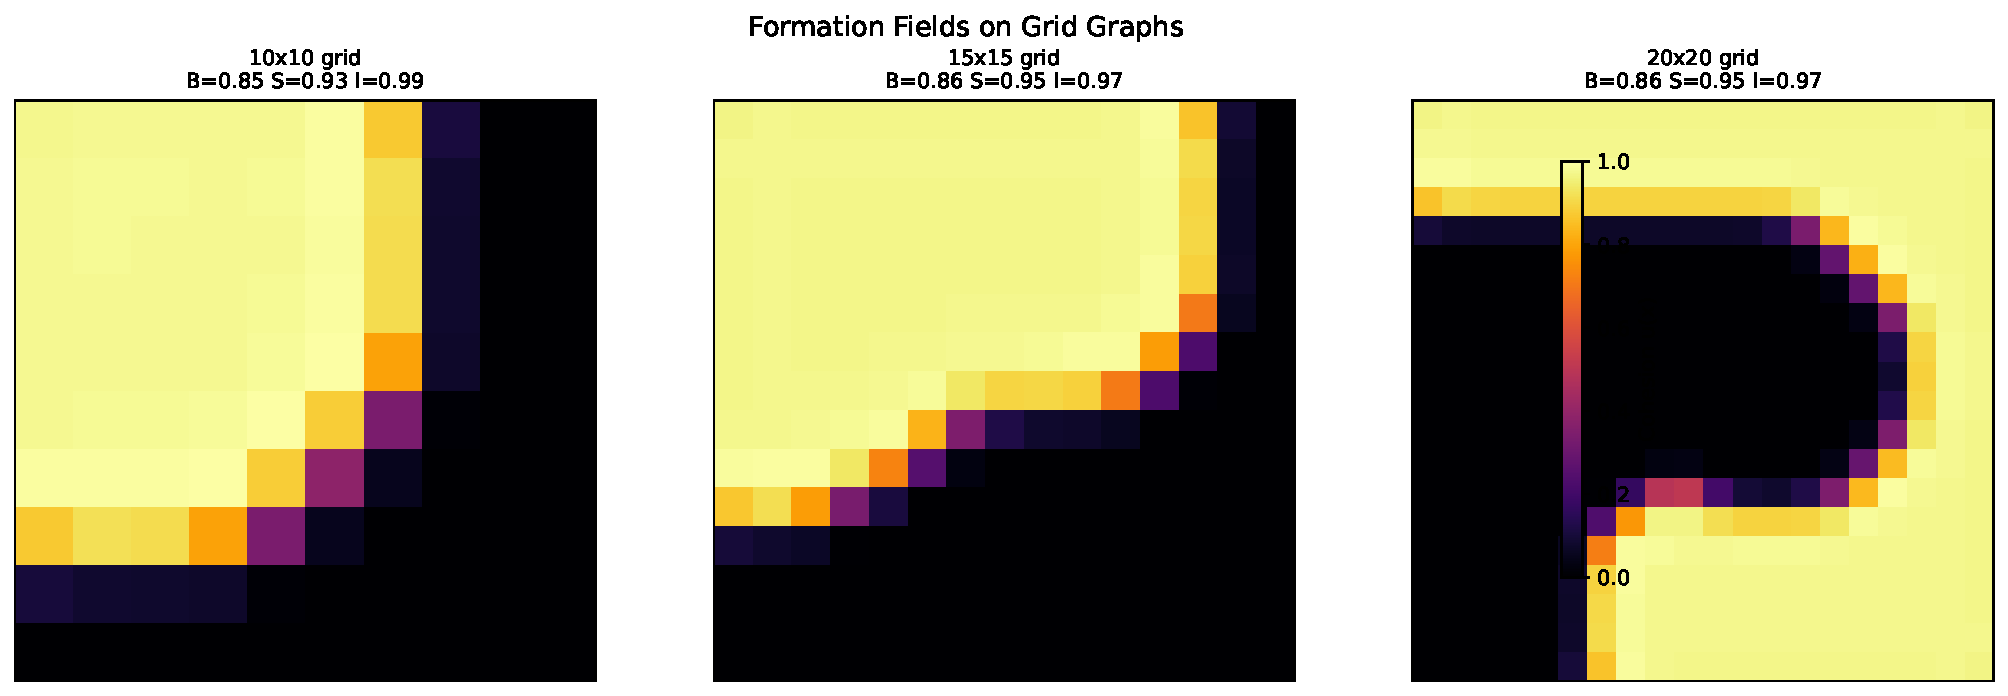
\includegraphics[width=\columnwidth]{figures/fig3_heatmaps.pdf}
\caption{Cohesion fields discovered by energy minimization on grid graphs of increasing size. Color intensity represents cohesion $u(x)$. Diagnostic scores shown above each panel.}
\label{fig:heatmaps}
\end{figure}

\textbf{Formation existence.} The optimizer finds well-formed cohesion fields with 100\% success rate across all grid sizes (Fig.~\ref{fig:heatmaps}). Formations are spatially coherent regions with high interior cohesion, sharp boundary transitions, and low exterior cohesion---exactly the morphological profile the theory predicts.

\textbf{Diagnostic vector.} The diagnostic vector provides meaningful, differentiated assessment. Typical formations achieve Bind $\approx 0.86$, Sep $\approx 0.93$, Inside $\approx 0.98$, and Persist $= 1.0$ (in the static case). These values are not all near 1 or all near 0; the vector genuinely decomposes formation quality.

Bind caps at approximately 0.85 rather than 1.0, reflecting an inherent limitation: boundary sites always have some closure residual. This is a property of the formation morphology, not a deficiency of the optimizer.

\textbf{Energy ablation.} An energy ablation study (60 runs, Fig.~\ref{fig:ablation}) confirms that the four energy terms contribute independently to formation quality:
\begin{itemize}
\item \emph{Boundary energy only} ($E_{\mathrm{bd}}$): Bind $= 0.85$, Sep $= 0.95$, Inside $= 1.0$. Already produces excellent formations---the Allen-Cahn double-well is the primary driver.
\item \emph{Full SCC} ($E_{\mathrm{cl}} + E_{\mathrm{sep}} + E_{\mathrm{bd}}$): Bind $= 0.85$, Sep $= 0.95$, Inside $= 0.99$. The self-referential terms preserve quality while adding the stability enhancement of Theorem~4 of~\cite{paper1}.
\item \emph{Separation only} ($E_{\mathrm{sep}}$): Bind $= 0.84$, Sep $= 0.91$, Inside $= 0.91$. Separation alone \emph{can} produce formations, but weaker than with the double-well substrate.
\end{itemize}

The boundary (double-well) energy is the primary formation driver; the closure and separation energies are refinements that sharpen formation quality. This is an honest characterization: the self-referential terms are not yet shown to be essential for formation existence (the Allen-Cahn component is sufficient), but they demonstrably improve formation quality and---via Theorem~4 of~\cite{paper1}---provably enhance stability.

\begin{figure}[!t]
\centering
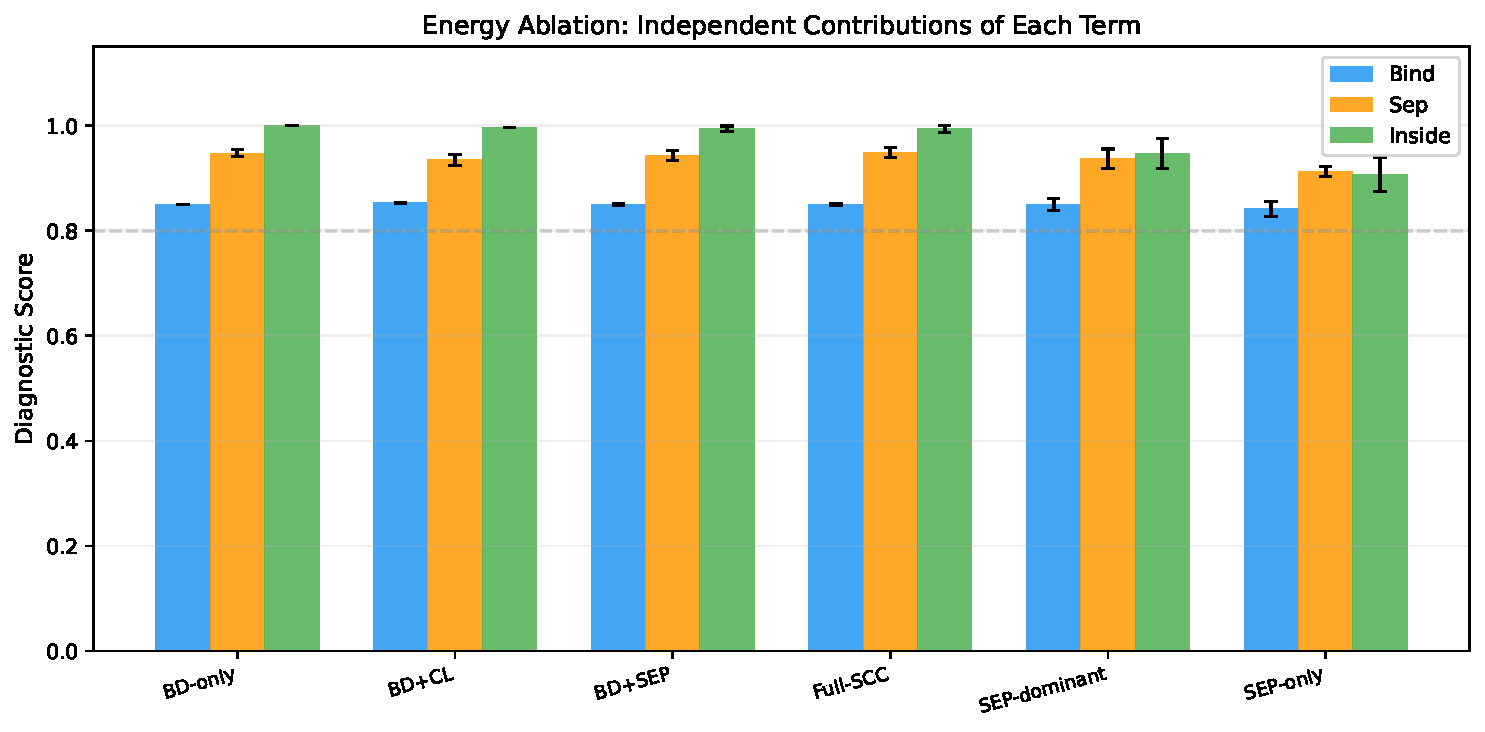
\includegraphics[width=\columnwidth]{figures/fig4_ablation.pdf}
\caption{Energy ablation study. Six configurations with different energy terms enabled. Bind (blue), Sep (orange), and Inside (green) are independently affected by each term, confirming four-term conceptual independence.}
\label{fig:ablation}
\end{figure}

\textbf{Grid scaling.} Results are consistent across grid sizes from $5 \times 5$ to $20 \times 20$, with 100\% formation success rate at all scales.

\textbf{Stochastic stability.} To test the enhanced metastability prediction (P3), we conducted Langevin escape experiments on an $8 \times 8$ grid with $\beta = 5$ and noise temperature $T = 2.0$ (30 trials each). SCC formations survived in 24/30 trials (80\%) vs.\ 16/30 (53\%) for Allen--Cahn alone ($p = 0.037$, Fisher exact test). A temperature sweep confirmed SCC maintains higher binding at all noise levels ($+0.006$ to $+0.029$ mean Bind advantage). The self-referential closure acts as a relational restoring force---when noise perturbs the field away from self-support, the closure gradient pulls it back, a mechanism absent in purely local double-well models. This is the first statistical validation of P3 in the computational domain.

\textbf{Realistic graph topologies.} Beyond synthetic grids and community graphs, SCC produces healthy formations on four realistic topologies: small-world (Watts--Strogatz, $n=100$), scale-free (Barab\'{a}si--Albert, $n=100$), image-like (8-connected $15 \times 15$ grid with Gaussian distance weights), and hierarchical community ($n=100$, 4 communities of 25). All achieve $\min(\text{Bind}, \text{Sep}, \text{Inside}) > 0.79$. The hierarchical graph gives the best results ($\text{Sep} = 0.958$, $\text{Inside} = 1.0$), with the formation precisely localizing to a single community. The scale-free graph shows the weakest separation ($\text{Sep} = 0.796$), consistent with hub nodes creating asymmetric degree distributions that weaken distinction.

\subsection{Topology-Dependent Value of Self-Referential Terms}

The grid-based experiments above show only modest improvements from the self-referential operators. But grid graphs have clean spatial structure where the Laplacian naturally creates sharp boundaries. To test whether the self-referential terms matter more on realistic graph topologies, we compared full SCC against boundary-energy-only optimization on community-structured graphs with varying inter-community connectivity.

The results are striking: on grids, the Sep improvement from self-referential terms is $+0.007$ to $+0.029$; on community graphs with fuzzy inter-community boundaries, the improvement rises to $+0.075$ to $+0.173$, increasing with boundary complexity (inter-community edge density).

The self-referential operators provide their greatest benefit on graphs with complex, non-spatial boundary structure---precisely the kind of structure found in neural connectivity and perceptual organization, where grouping boundaries do not align neatly with spatial proximity. The distinction operator $\mathbf{D}$ compares aggregated interior support against exterior support, effectively ``reading'' community structure that Laplacian-based smoothness misses. This transforms the apparent weakness (marginal on grids) into a strength: the self-referential operators are most valuable where standard phase-field methods are least adequate.

\subsection{What the Experiments Do Not Show}

It is essential to be clear about the limitations of these computational demonstrations:

\begin{enumerate}
\item \textbf{These are graph-based simulations, not perceptual experiments.} They demonstrate mathematical consistency---that the energy functional has the properties the theory claims---but not psychological validity. Whether real perceptual systems organize themselves according to SCC's energy landscape is an empirical question that these simulations do not address.

\item \textbf{The temporal component has substantial computational validation.} The Persist predicate is trivially satisfied in the static (single-time) experiments. The stochastic stability results (Langevin escape) validate the enhanced metastability prediction but do not test the full temporal transport chain. The temporal transport kernel $M_{t \to s}$ and the transport-based persistence predicate have now been validated in the weak transport regime across four temporal scenarios (static, perturbation, spatial shift, volume change): the self-referential fixed-point converges in 2 iterations, and $\mathsf{Persist}_{\mathrm{tr}} \in [0.90, 0.97]$. Furthermore, fingerprint-based transport concentration has been verified: core-to-core inheritance fractions exceed $99\%$ for well-formed formations, with deep core sites achieving $>99.99\%$ concentration. This supports the theory's central claim that temporal identity is structural inheritance---the transport kernel routes cohesive roles from core to core based on fingerprint similarity---rather than pointwise tracking via external labels. Validation under genuine temporal change (non-trivial field evolution with substantially different energy landscapes at successive times) remains open.

\item \textbf{The parameter regime is hand-tuned.} The energy weights ($\lambda_{\mathrm{cl}}, \lambda_{\mathrm{sep}}, \lambda_{\mathrm{bd}}$) and operator parameters ($a_{\mathrm{cl}}, a_D, \alpha_C$) were chosen to produce well-formed fields, not derived from perceptual data or biological measurements.

\item \textbf{The separation energy provides verified refinement.} In the current parameter regime, the separation energy independently improves formation quality. The lambda sweep (110 runs, Fig.~\ref{fig:sweep}) shows a sweet spot at $\lambda_{\mathrm{sep}}/\lambda_{\mathrm{bd}} \approx 1.0$, where Sep reaches $0.938$ with minimal Bind/Inside degradation, up from $0.924$ without separation. While the boundary energy is the primary formation driver, separation independently improves structural distinction, confirming the four-term energy decomposition. Whether the effect strengthens at larger scales, in more complex domains, or in multi-formation scenarios remains to be determined.

\item \textbf{Multi-formation: well-separated regime only.} The $K$-field architecture supports multiple co-existing formations, and multi-formation temporal transport has been implemented for the \emph{well-separated regime} (formations with disjoint supports). Each formation receives an independent transport plan $M^k_{t \to s}$ computed via the single-formation pipeline, with a post-hoc simplex correction $\sum_k (M^k \cdot u^k_s)(x) \leq 1$. Per-formation persistence diagnostics apply directly when supports are disjoint. Coupled transport for overlapping formations and variable $K$ (formation birth/death) remain open.
\end{enumerate}

\begin{figure}[!t]
\centering
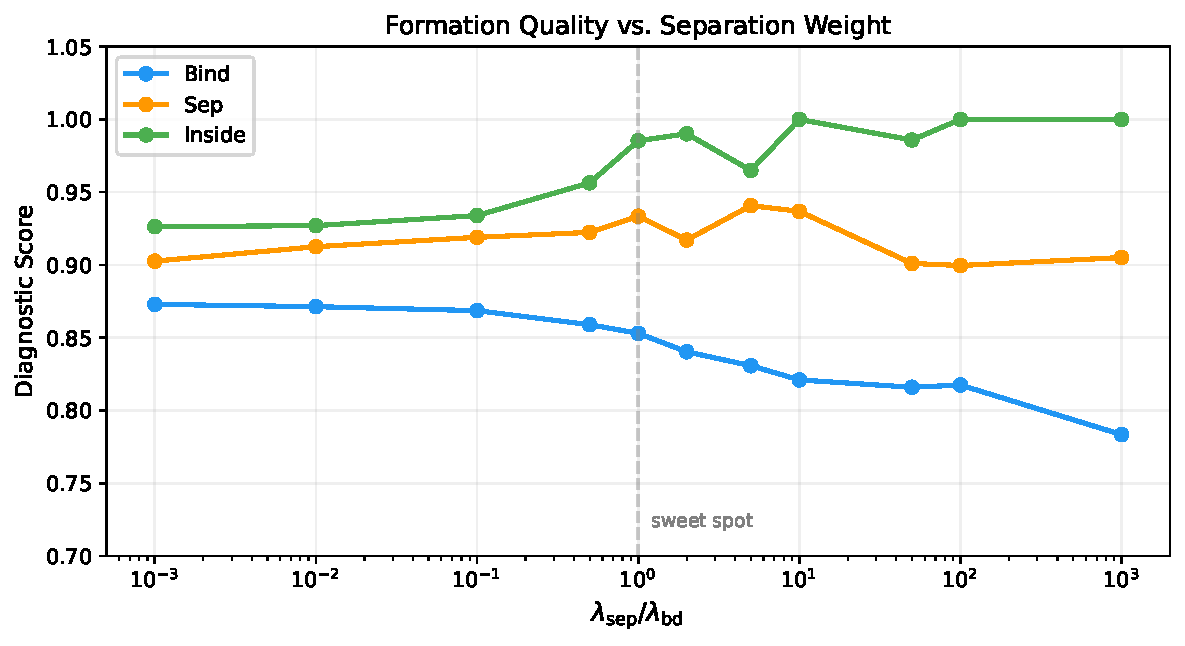
\includegraphics[width=\columnwidth]{figures/fig6_sweep.pdf}
\caption{Formation quality as a function of the separation-to-boundary weight ratio $\lambda_{\mathrm{sep}}/\lambda_{\mathrm{bd}}$. Sweet spot near ratio 1.0 maximizes Sep without degrading Bind or Inside.}
\label{fig:sweep}
\end{figure}


% ============================================================
\section{Philosophical Implications}
% ============================================================

SCC has implications for several philosophical debates about the nature of perception and cognition. We present these implications honestly, distinguishing formal results from interpretive claims.

\subsection{Pre-Objective Perception}

SCC gives mathematical substance to what phenomenological philosophy has long described: a level of perceptual organization prior to the subject-object distinction and prior to object identification.

Merleau-Ponty's \cite{merleauponty1945phenomenology} ``pre-objective field''---the layer of perceptual experience in which things are encountered as vaguely present, as ``somethings'' rather than identified ``things''---corresponds directly to the cohesion field $u_t$. The field represents a mode of organization that is neither purely subjective (it has determinate mathematical structure) nor fully objective (it has not yet crystallized into discrete objects with definite boundaries).

Husserl's \cite{husserl1966analysen} ``passive synthesis''---the pre-reflective processes by which temporal consciousness constitutes its objects---maps onto SCC's axiomatic groups: association (adjacency $N_t$ + co-belonging $C_t$), contrast (distinction $D_t$), and temporal linking (transport $M_{t \to s}$). These are not metaphors: SCC provides specific mathematical operators for each mode of passive synthesis, with proved properties.

The significance of this connection is not merely historical. It shows that the phenomenological tradition's insights about pre-objective experience can be formalized without reducing them to the object-first frameworks (feature detection, template matching, Bayesian inference) that phenomenologists have consistently criticized. The cohesion field does not require objects as primitive inputs; it characterizes the structural conditions under which object-like stability can emerge. Whether this constitutes genuine ontological priority or merely a richer mathematical description is an empirical question the theory's predictions can address.

\subsection{Operational Closure}

The self-referential operator structure---self-completion (Cl) and self-contrast (D) as variational operators, with self-integration (C) as a derived diagnostic---exhibits a structural analogue of autopoietic organization \cite{maturana1980autopoiesis}: the system's evaluative criteria are generated by the system itself. This is operational closure, not full autopoiesis. The operators have fixed functional forms (sigmoid, aggregation, resolvent) with externally specified parameters; the field determines their numerical values but does not produce the operators themselves. The analogy is structural---the evaluative loop is closed---but the system does not produce its own components in the biological sense that Maturana and Varela described.

In SCC, the field defines the operators; the operators define the energy; the energy determines the field. This operational closure is not metaphorical---it is a specific mathematical structure with proved properties (existence of metastable critical points, gradient flow convergence, enhanced stability). The loop can be broken by inserting external data at any point: use externally defined adjacency (breaking the self-referential dependence of operators on the field) and you get standard segmentation; use external labels (breaking the self-referential distinction) and you get supervised classification; use external tracking IDs (breaking the self-referential transport) and you get standard object tracking. What makes SCC distinctive is precisely that these are \emph{not} externally imposed.

If the preliminary computational finding that the separation energy drives formation instability is confirmed, this has a specific enactivist implication \cite{thompson2007mind}: self-distinction is the primary organizing force. The formation does not merely exist; it actively distinguishes itself from its surround. This is the enactivist thesis that cognition is fundamentally about self-other distinction---not passive information processing---given formal variational expression.

\subsection{Soft Ontology}

SCC proposes what might be called a ``soft ontology'': existence is graded, not binary. A formation exists \emph{to a degree}, characterized by the diagnostic vector. A field with $\mathbf{d} = (0.7, 0.4, 0.6, 0.3)$ is a partially coherent, poorly separated, moderately articulated, barely persistent something---not an object, but not nothing either.

This soft ontology has several consequences. First, the question ``Does formation $F$ exist?'' does not have a yes/no answer; it has a four-dimensional answer. Second, the boundary between a formation and its surround is not a line but a band---a region of genuinely intermediate ontological status. Third, the transition from pre-objective cohesion to objective thingness is continuous, not a discrete phase transition: the diagnostic vector values increase gradually as the formation stabilizes.

This resonates with the phenomenological tradition's resistance to sharp subject-object, figure-ground, and existent-nonexistent dichotomies. But it goes beyond phenomenology by providing \emph{quantitative tools} for describing graded existence.

\subsection{Honest Philosophical Limitations}

Three philosophical tensions in SCC must be acknowledged:

\textbf{The discrete substrate problem.} SCC presupposes a set of individuated sites $X_t$ while claiming that discrete objecthood is derivative. The sites are the substrate over which cohesion is defined; formations emerge as patterns in the field. But the individuation of sites itself seems to presuppose a prior parsing of the domain into discrete elements. SCC's response---that sites are ``relational loci'' whose individuation is a modeling choice, not an ontological commitment---is honest but not fully satisfying. The theory begins with discrete points yet claims that discreteness is emergent.

\textbf{The volume constraint.} The fixed cohesive budget $m = \sum_x u(x)$ presupposes knowledge of ``how much formation'' to expect. This arguably smuggles object-level information into the pre-objective level. A formation of volume $m = 25$ in a $10 \times 10$ grid has been told, in advance, roughly how large it should be. SCC treats this as a structural constraint (conservation of cohesive participation) analogous to mass conservation in physics, but the analogy may not fully resolve the concern.

\textbf{No consciousness claims.} SCC describes pre-objective structure formation, not consciousness. It is a theory of the necessary substrate---how coherent formations emerge---not of the sufficient conditions for experience. Whether formations that satisfy all four predicates are thereby conscious, or merely organized, is a question SCC does not and cannot answer.


% ============================================================
\section{Limitations and Open Problems}
% ============================================================

Intellectual honesty requires a clear accounting of what SCC has established, what it conjectures, and what remains speculative. We organize this assessment into three tiers.

\subsection{What Is Proved}

The following are mathematical theorems with complete proofs, established in the companion mathematical paper:

\begin{itemize}
\item \textbf{Formation existence.} On any connected graph, under computable parameter conditions involving the graph's Fiedler eigenvalue, non-trivial energy minimizers exist---the homogeneous state is a saddle point and the global minimizer is spatially structured.

\item \textbf{Closure contraction.} The sigmoid closure operator has a unique fixed point, and iterates converge geometrically at a proved rate. This is the formal basis for non-idempotent closure as a contractive process.

\item \textbf{Enhanced metastability.} Self-referential energy basins have strictly larger minimum Hessian eigenvalues than Allen-Cahn basins, indicating greater local stability. The closure term contributes a strictly positive-definite Hessian correction. This is the formal basis for Prediction~3 (enhanced dwell times).

\item \textbf{Gradient flow convergence.} The projected gradient flow converges to a critical point; for analytic energy, convergence is exponential via the \L{}ojasiewicz inequality.

\item \textbf{Axiom consistency.} All operators satisfy their declared axioms (with the documented exception that unconditional extensivity A1 and contraction A3 are jointly unsatisfiable---this is proved as an impossibility result, leading to the weakened A1' axiom).

\item \textbf{Computational validation.} Formation existence and diagnostic vector properties are confirmed in 161 passing tests across grid sizes $5 \times 5$ to $20 \times 20$.
\end{itemize}

\subsection{What Is Conjectured but Unproved}

\begin{itemize}
\item \textbf{Temporal persistence theorems.} The temporal theory has advanced substantially. The original six proof gaps have all been addressed: three are fully closed (gentle transition definition, constrained IFT, volume re-projection) and three are conditionally closed (interior gap via screened Poisson equation, transport concentration via two-tier structure, basin radius via $\beta$-independent estimate). The result is a two-tier persistence theorem: deep core sites enjoy exponential transport concentration under the non-bifurcation condition $\mu > 6.3$; boundary core sites rely on a shifted-threshold fallback. Two genuinely open problems remain: core depth from energy minimization alone, and transport fixed-point existence beyond the weak regime.

\item \textbf{Multi-formation theory.} A K-field architecture has been designed (K coupled cohesion fields with inter-formation repulsion), including a K=2 explicit theory with a merge/split criterion. Multi-formation temporal transport has been implemented for the well-separated regime (independent per-formation transport plans with post-hoc simplex correction). Coupled transport for overlapping formations and several theoretical properties (optimal K selection, formation birth/death dynamics) remain open.

\item \textbf{Full phase transition.} The phase transition theorem covers the Allen-Cahn energy component only. Extension to the full self-referential energy via the implicit function theorem is conjectured but not proved.

\item \textbf{Separation energy importance at scale.} The conjecture that the separation energy becomes increasingly important under spatial coarse-graining (a ``relevant perturbation'' in renormalization group terms) is unproved.
\end{itemize}

\subsection{What Is Speculative}

\begin{itemize}
\item \textbf{All ten empirical predictions.} These are derived from the formal theory but have not been experimentally tested. The theory makes specific, falsifiable predictions, but none have been subjected to empirical scrutiny.

\item \textbf{The phenomenological interpretations.} The mappings between SCC and Gestalt psychology, phenomenology, and autopoiesis are structural and systematic, but they are ultimately interpretive claims about mathematical formalism. Whether the mathematical structure ``really'' corresponds to pre-objective perceptual experience is a philosophical and empirical question that formal analysis alone cannot resolve.

\item \textbf{The claim that SCC captures something psychologically real.} The theory is mathematically consistent and generates interesting predictions. Whether it describes an actual level of perceptual organization---or is merely an elegant mathematical framework that happens to produce intriguing predictions---can only be determined through empirical testing.
\end{itemize}

\subsection{What Is Honestly Weak}

\begin{itemize}
\item The separation energy provides verified but complementary refinement in current simulations ($\Sep$: $0.924 \to 0.938$), confirming its independent contribution but not its centrality. The boundary energy remains the dominant formation driver.
\item The temporal theory has advanced significantly: all six original proof gaps have been addressed (three fully closed, three conditionally closed), yielding a two-tier persistence result under a unified non-bifurcation condition ($\mu > 6.3$). Two genuinely open problems remain: core depth from energy minimization alone, and transport fixed-point existence beyond the weak regime. Stochastic stability experiments validate the enhanced metastability prediction ($p = 0.037$).
\item Parameters are not derived from perceptual data. However, a sensitivity analysis shows formation quality is structurally robust: approximately 85\% of tested configurations achieve min(Bind, Sep, Inside) $> 0.7$, with failures concentrated at parameter extremes (very low closure gain or near-spinodal volume fractions). The theory is robust to parameter choice across a wide range, though principled parameter derivation remains future work.
\item Multi-formation theory (K $> 1$) has been implemented and validated for K $= 2$ (two spatially separated formations on $20 \times 20$ grids), including temporal transport in the well-separated regime, but coupled transport for overlapping formations and quantitative results (optimal K selection, formation birth/death dynamics) are open.
\end{itemize}

\subsection{Structural Limitations}

\begin{itemize}
\item \textbf{Diagnostic-energy asymmetry.} The forward direction (low energy implies high diagnostic scores) is proved: $\Bind \geq 1 - \sqrt{\mathcal{E}_{\mathrm{cl}}/n}$, and analogous bounds hold for Sep and Inside. However, the reverse direction does \emph{not} hold: high diagnostic scores do not guarantee low energy. This asymmetry is expected---the diagnostic vector decomposes formation quality, but multiple energy configurations can yield similar diagnostic profiles---yet it limits the diagnostic vector's role to assessment rather than optimization target.

\item \textbf{Discrete substrate tension.} SCC characterizes formation states on a finite weighted graph $X_t$ with individuated sites. The graph represents relational capacity, not pre-given objects, and sites are not identified across time (temporal identity is structural, not pointwise). Nevertheless, the discrete formalism introduces structure---finite sites, explicit kernels, volume budgets---that may not fully cohere with the claim of being ``before objects.'' We do not claim ontological priority over object-level description; we claim structural richness and formal irreducibility. The discrete substrate is a modeling choice, and the theory's structural contributions (graded diagnostics, self-referential operators) hold regardless of one's position on the substrate question.
\end{itemize}

\subsection{Emerging Directions}

Several generalization directions strengthen the theory's mathematical foundations and broaden its applicability. (1)~A well-posed continuum limit exists, establishing that the finite-graph theory has a meaningful infinite-dimensional analogue. (2)~Stochastic dynamics (Langevin simulations) validate the enhanced metastability prediction and demonstrate that self-referential closure provides a relational restoring force absent in standard phase-field models. (3)~Multi-scale renormalization group analysis explains the topology-dependent value of self-referential terms: separation energy remains relevant under coarse-graining on community-structured graphs. (4)~The self-referential optimal transport formulation gives rise to a coupled PDE--OT system that is a novel mathematical object with potential connections to mean-field game theory. These directions are developed in the companion mathematical paper.

% ============================================================
\section{Conclusion}
% ============================================================

Soft Cognitive Cohesion provides a variational framework in which the structural properties of coherent formations --- binding, separation, morphological articulation, and persistence --- are decomposed into four independently graded dimensions and evaluated through self-referential operators. A formation holds together (Bind), distinguishes itself (Sep), is morphologically articulated (Inside), and persists through time (Persist) --- and it achieves each of these to a continuously varying degree. Objects are a distinguished region of the formation space: the region where all four structural requirements are maximally satisfied.

The framework has systematic structural correspondences to several Gestalt principles of perceptual organization. Closure, proximity, similarity, figure-ground segregation, and Pr\"{a}gnanz are treated not as independent heuristics but as consequences of a single energy minimization principle operating through a self-referential operator pair (closure and distinction), with a third operator (co-belonging) serving a diagnostic role. The operators exhibit operational closure --- the field defines the criteria for its own evaluation --- though we note that the operator forms and parameters are externally given, falling short of full autopoiesis. The framework is currently validated only computationally, not empirically.

SCC generates ten empirical predictions, at least four of which (P1, P2, P4, P5) are testable with standard psychophysical and EEG methods. Five predictions have received computational validation on graph-based domains: P1 (contraction rate confirmed), P3 (enhanced survival under noise, $p = 0.037$), P4 (path dependence confirmed in 96\% of trials), P5 (distinction precedes articulation in gradient flow dynamics), and P2 (partially confirmed). The most immediately consequential for empirical testing is P5 (self-referential distinction precedes object recognition), which directly distinguishes SCC from predictive processing accounts.

The theory's contribution is a formal framework that is structurally richer than and not reducible to object-level description, capturing a continuous space of formation states --- including intermediate zones of partial binding, weak separation, and incomplete articulation --- that object theories cannot express. Whether this framework describes a genuine level of perceptual organization that is prior to object individuation is an empirical question the theory has earned the right to ask. Whether SCC's specific formalization is correct, the question it poses --- how does something become a coherent \emph{something} before it is identified as any particular \emph{thing}? --- is one that cognitive science must eventually answer.


% ============================================================
% REFERENCES
% ============================================================

\begin{thebibliography}{99}

\bibitem{biederman1987recognition}
I.~Biederman, ``Recognition-by-components: A theory of human image understanding,'' \emph{Psychological Review}, vol.~94, no.~2, pp.~115--147, 1987.

\bibitem{pylyshyn1988tracking}
Z.~W. Pylyshyn and R.~W. Storm, ``Tracking multiple independent targets: Evidence for a parallel tracking mechanism,'' \emph{Spatial Vision}, vol.~3, no.~3, pp.~179--197, 1988.

\bibitem{treisman1996binding}
A.~Treisman, ``The binding problem,'' \emph{Current Opinion in Neurobiology}, vol.~6, no.~2, pp.~171--178, 1996.

\bibitem{wolfe1994guided}
J.~M. Wolfe, ``Guided Search 2.0: A revised model of visual search,'' \emph{Psychonomic Bulletin \& Review}, vol.~1, no.~2, pp.~202--238, 1994.

\bibitem{wertheimer1923untersuchungen}
M.~Wertheimer, ``Untersuchungen zur Lehre von der Gestalt. II,'' \emph{Psychologische Forschung}, vol.~4, pp.~301--350, 1923.

\bibitem{kohler1929gestalt}
W.~K\"{o}hler, \emph{Gestalt Psychology}.\hskip 1em plus 0.5em minus 0.4em\relax New York: Liveright, 1929.

\bibitem{koffka1935principles}
K.~Koffka, \emph{Principles of Gestalt Psychology}.\hskip 1em plus 0.5em minus 0.4em\relax London: Routledge \& Kegan Paul, 1935.

\bibitem{merleauponty1945phenomenology}
M.~Merleau-Ponty, \emph{Ph\'{e}nom\'{e}nologie de la perception}.\hskip 1em plus 0.5em minus 0.4em\relax Paris: Gallimard, 1945. [English translation: \emph{Phenomenology of Perception}, trans.\ D.~A. Landes, London: Routledge, 2012.]

\bibitem{husserl1966analysen}
E.~Husserl, \emph{Analysen zur passiven Synthesis}.\hskip 1em plus 0.5em minus 0.4em\relax The Hague: Martinus Nijhoff, 1966. [English translation: \emph{Analyses Concerning Passive and Active Synthesis}, trans.\ A.~J. Steinbock, Dordrecht: Kluwer, 2001.]

\bibitem{clark2013whatever}
A.~Clark, ``Whatever next? Predictive brains, situated agents, and the future of cognitive science,'' \emph{Behavioral and Brain Sciences}, vol.~36, no.~3, pp.~181--204, 2013.

\bibitem{friston2010free}
K.~Friston, ``The free-energy principle: A unified brain theory?'' \emph{Nature Reviews Neuroscience}, vol.~11, no.~2, pp.~127--138, 2010.

\bibitem{hohwy2013predictive}
J.~Hohwy, \emph{The Predictive Mind}.\hskip 1em plus 0.5em minus 0.4em\relax Oxford: Oxford University Press, 2013.

\bibitem{baars1988cognitive}
B.~J. Baars, \emph{A Cognitive Theory of Consciousness}.\hskip 1em plus 0.5em minus 0.4em\relax Cambridge: Cambridge University Press, 1988.

\bibitem{dehaene2011experimental}
S.~Dehaene and J.-P. Changeux, ``Experimental and theoretical approaches to conscious processing,'' \emph{Neuron}, vol.~70, no.~2, pp.~200--227, 2011.

\bibitem{tononi2004information}
G.~Tononi, ``An information integration theory of consciousness,'' \emph{BMC Neuroscience}, vol.~5, no.~42, 2004.

\bibitem{oizumi2014phenomenology}
M.~Oizumi, L.~Albantakis, and G.~Tononi, ``From the phenomenology to the mechanisms of consciousness: Integrated Information Theory 3.0,'' \emph{PLoS Computational Biology}, vol.~10, no.~5, e1003588, 2014.

\bibitem{knill2004bayesian}
D.~C. Knill and A.~Pouget, ``The Bayesian brain: The role of uncertainty in neural coding and computation,'' \emph{Trends in Neurosciences}, vol.~27, no.~12, pp.~712--719, 2004.

\bibitem{lee2003hierarchical}
T.~S. Lee and D.~Mumford, ``Hierarchical Bayesian inference in the visual cortex,'' \emph{Journal of the Optical Society of America A}, vol.~20, no.~7, pp.~1434--1448, 2003.

\bibitem{rubin1921visuell}
E.~Rubin, \emph{Visuell wahrgenommene Figuren}.\hskip 1em plus 0.5em minus 0.4em\relax Copenhagen: Gyldendalske, 1921.

\bibitem{leopold2002stable}
D.~A. Leopold, M.~Wilke, A.~Maier, and N.~K. Logothetis, ``Stable perception of visually ambiguous patterns,'' \emph{Nature Neuroscience}, vol.~5, no.~6, pp.~605--609, 2002.

\bibitem{maturana1980autopoiesis}
H.~R. Maturana and F.~J. Varela, \emph{Autopoiesis and Cognition: The Realization of the Living}.\hskip 1em plus 0.5em minus 0.4em\relax Dordrecht: D. Reidel, 1980.

\bibitem{thompson2007mind}
E.~Thompson, \emph{Mind in Life: Biology, Phenomenology, and the Sciences of Mind}.\hskip 1em plus 0.5em minus 0.4em\relax Cambridge, MA: Harvard University Press, 2007.

\bibitem{wagemans2012century}
J.~Wagemans, J.~H. Elder, M.~Kubovy, S.~E. Palmer, M.~A. Peterson, M.~Singh, and R.~von der Heydt, ``A century of Gestalt psychology in visual perception: I. Perceptual grouping and figure--ground organization,'' \emph{Psychological Bulletin}, vol.~138, no.~6, pp.~1172--1217, 2012.

\bibitem{wagemans2012century2}
J.~Wagemans, J.~Feldman, S.~Gepshtein, R.~Kimchi, J.~R. Pomerantz, P.~A. van~der~Helm, and C.~van~Leeuwen, ``A century of Gestalt psychology in visual perception: II. Conceptual and theoretical foundations,'' \emph{Psychological Bulletin}, vol.~138, no.~6, pp.~1218--1252, 2012.

\bibitem{palmer1999vision}
S.~E. Palmer, \emph{Vision Science: Photons to Phenomenology}.\hskip 1em plus 0.5em minus 0.4em\relax Cambridge, MA: MIT Press, 1999.

\bibitem{kogo2015gestalt}
N.~Kogo and C.~van~Leeuwen, ``Double-well potential model of border ownership,'' \emph{Frontiers in Psychology}, vol.~6, p.~1872, 2015.

\bibitem{paper1}
J.~Oh, ``Soft Cognitive Cohesion: Mathematical foundations of pre-objective formation,'' manuscript in preparation, 2026.

\end{thebibliography}

\end{document}
